% Options for packages loaded elsewhere
\PassOptionsToPackage{unicode}{hyperref}
\PassOptionsToPackage{hyphens}{url}
%
\documentclass[
  11pt,
  a4paper,
]{book}
\usepackage[]{mathpazo}
\usepackage{amssymb,amsmath}
\usepackage{ifxetex,ifluatex}
\ifnum 0\ifxetex 1\fi\ifluatex 1\fi=0 % if pdftex
  \usepackage[T1]{fontenc}
  \usepackage[utf8]{inputenc}
  \usepackage{textcomp} % provide euro and other symbols
\else % if luatex or xetex
  \usepackage{unicode-math}
  \defaultfontfeatures{Scale=MatchLowercase}
  \defaultfontfeatures[\rmfamily]{Ligatures=TeX,Scale=1}
\fi
% Use upquote if available, for straight quotes in verbatim environments
\IfFileExists{upquote.sty}{\usepackage{upquote}}{}
\IfFileExists{microtype.sty}{% use microtype if available
  \usepackage[]{microtype}
  \UseMicrotypeSet[protrusion]{basicmath} % disable protrusion for tt fonts
}{}
\makeatletter
\@ifundefined{KOMAClassName}{% if non-KOMA class
  \IfFileExists{parskip.sty}{%
    \usepackage{parskip}
  }{% else
    \setlength{\parindent}{0pt}
    \setlength{\parskip}{6pt plus 2pt minus 1pt}}
}{% if KOMA class
  \KOMAoptions{parskip=half}}
\makeatother
\usepackage{xcolor}
\IfFileExists{xurl.sty}{\usepackage{xurl}}{} % add URL line breaks if available
\IfFileExists{bookmark.sty}{\usepackage{bookmark}}{\usepackage{hyperref}}
\hypersetup{
  pdftitle={Trabajo final Estadística Avanzada},
  pdfauthor={Carlos Alberto Murillo M; Luz Stella Florez; Diana Carolina Benjumea; Cindy Guerra},
  pdfkeywords={Maestria Ciencia Datos, ,},
  hidelinks,
  pdfcreator={LaTeX via pandoc}}
\urlstyle{same} % disable monospaced font for URLs
\usepackage[margin=1in]{geometry}
\usepackage{color}
\usepackage{fancyvrb}
\newcommand{\VerbBar}{|}
\newcommand{\VERB}{\Verb[commandchars=\\\{\}]}
\DefineVerbatimEnvironment{Highlighting}{Verbatim}{commandchars=\\\{\}}
% Add ',fontsize=\small' for more characters per line
\usepackage{framed}
\definecolor{shadecolor}{RGB}{248,248,248}
\newenvironment{Shaded}{\begin{snugshade}}{\end{snugshade}}
\newcommand{\AlertTok}[1]{\textcolor[rgb]{0.94,0.16,0.16}{#1}}
\newcommand{\AnnotationTok}[1]{\textcolor[rgb]{0.56,0.35,0.01}{\textbf{\textit{#1}}}}
\newcommand{\AttributeTok}[1]{\textcolor[rgb]{0.77,0.63,0.00}{#1}}
\newcommand{\BaseNTok}[1]{\textcolor[rgb]{0.00,0.00,0.81}{#1}}
\newcommand{\BuiltInTok}[1]{#1}
\newcommand{\CharTok}[1]{\textcolor[rgb]{0.31,0.60,0.02}{#1}}
\newcommand{\CommentTok}[1]{\textcolor[rgb]{0.56,0.35,0.01}{\textit{#1}}}
\newcommand{\CommentVarTok}[1]{\textcolor[rgb]{0.56,0.35,0.01}{\textbf{\textit{#1}}}}
\newcommand{\ConstantTok}[1]{\textcolor[rgb]{0.00,0.00,0.00}{#1}}
\newcommand{\ControlFlowTok}[1]{\textcolor[rgb]{0.13,0.29,0.53}{\textbf{#1}}}
\newcommand{\DataTypeTok}[1]{\textcolor[rgb]{0.13,0.29,0.53}{#1}}
\newcommand{\DecValTok}[1]{\textcolor[rgb]{0.00,0.00,0.81}{#1}}
\newcommand{\DocumentationTok}[1]{\textcolor[rgb]{0.56,0.35,0.01}{\textbf{\textit{#1}}}}
\newcommand{\ErrorTok}[1]{\textcolor[rgb]{0.64,0.00,0.00}{\textbf{#1}}}
\newcommand{\ExtensionTok}[1]{#1}
\newcommand{\FloatTok}[1]{\textcolor[rgb]{0.00,0.00,0.81}{#1}}
\newcommand{\FunctionTok}[1]{\textcolor[rgb]{0.00,0.00,0.00}{#1}}
\newcommand{\ImportTok}[1]{#1}
\newcommand{\InformationTok}[1]{\textcolor[rgb]{0.56,0.35,0.01}{\textbf{\textit{#1}}}}
\newcommand{\KeywordTok}[1]{\textcolor[rgb]{0.13,0.29,0.53}{\textbf{#1}}}
\newcommand{\NormalTok}[1]{#1}
\newcommand{\OperatorTok}[1]{\textcolor[rgb]{0.81,0.36,0.00}{\textbf{#1}}}
\newcommand{\OtherTok}[1]{\textcolor[rgb]{0.56,0.35,0.01}{#1}}
\newcommand{\PreprocessorTok}[1]{\textcolor[rgb]{0.56,0.35,0.01}{\textit{#1}}}
\newcommand{\RegionMarkerTok}[1]{#1}
\newcommand{\SpecialCharTok}[1]{\textcolor[rgb]{0.00,0.00,0.00}{#1}}
\newcommand{\SpecialStringTok}[1]{\textcolor[rgb]{0.31,0.60,0.02}{#1}}
\newcommand{\StringTok}[1]{\textcolor[rgb]{0.31,0.60,0.02}{#1}}
\newcommand{\VariableTok}[1]{\textcolor[rgb]{0.00,0.00,0.00}{#1}}
\newcommand{\VerbatimStringTok}[1]{\textcolor[rgb]{0.31,0.60,0.02}{#1}}
\newcommand{\WarningTok}[1]{\textcolor[rgb]{0.56,0.35,0.01}{\textbf{\textit{#1}}}}
\usepackage{graphicx,grffile}
\makeatletter
\def\maxwidth{\ifdim\Gin@nat@width>\linewidth\linewidth\else\Gin@nat@width\fi}
\def\maxheight{\ifdim\Gin@nat@height>\textheight\textheight\else\Gin@nat@height\fi}
\makeatother
% Scale images if necessary, so that they will not overflow the page
% margins by default, and it is still possible to overwrite the defaults
% using explicit options in \includegraphics[width, height, ...]{}
\setkeys{Gin}{width=\maxwidth,height=\maxheight,keepaspectratio}
% Set default figure placement to htbp
\makeatletter
\def\fps@figure{htbp}
\makeatother
\setlength{\emergencystretch}{3em} % prevent overfull lines
\providecommand{\tightlist}{%
  \setlength{\itemsep}{0pt}\setlength{\parskip}{0pt}}
\setcounter{secnumdepth}{-\maxdimen} % remove section numbering
\usepackage{booktabs}
\usepackage{longtable}
\usepackage{array}
\usepackage{multirow}
\usepackage{wrapfig}
\usepackage{float}
\usepackage{colortbl}
\usepackage{pdflscape}
\usepackage{tabu}
\usepackage{threeparttable}
\usepackage{threeparttablex}
\usepackage[normalem]{ulem}
\usepackage{makecell}
\usepackage{xcolor}
\usepackage[]{natbib}
\bibliographystyle{apsr}

\title{Trabajo final Estadística Avanzada}
\author{Carlos Alberto Murillo M \and Luz Stella Florez \and Diana Carolina Benjumea \and Cindy Guerra}
\date{noviembre 28, 2020}

\begin{document}
\frontmatter
\maketitle

{
\setcounter{tocdepth}{2}
\tableofcontents
}
\mainmatter
\hypertarget{abstract}{%
\chapter*{Abstract}\label{abstract}}
\addcontentsline{toc}{chapter}{Abstract}

Este documento analiza los impactos de las variables macroeconómicas en
los costos y gastos de empresas del sector ``Extracción de oro y otros
metales preciosos''. Para el análisis, se tomaron los datos de los años:
2017, 2018 y 2019. El código de este trabajo se encuentra almacenado en
el repositorio de Github:
\url{https://github.com/cabymetal/TrabajoFinal_estadisticos_avanzados}.

\hypertarget{objetivos-y-lineamientos}{%
\chapter{Objetivos y Lineamientos}\label{objetivos-y-lineamientos}}

Caracterizar las relaciones entre algunos indicadores macroeconómicos y
los costos y gastos de ventas de las empresas colombianas vigiladas por
la SuperSociedades.

Lineamientos:

\begin{enumerate}
\def\labelenumi{\arabic{enumi}.}
\item
  Con ayuda de un modelo lineal modele cree un modelo o varios modelos
  que permitan caracterizar la relación entre las variables PIB,
  Inflación, Desempleo, Tasa de Cambio, Balance Fiscal, Balance en
  Cuenta Corriente, Tasa de intervención, TRM y los costos y gastos de
  ventas.
\item
  Se debe escoger mínimo un tipo de empresas (Clasificación Industrial
  Internacional Uniforme) que tenga más de 20 empresas y tomar al menos
  los últimos tres años de información disponible.
\item
  Se debe evaluar el ajuste y la capacidad predictiva.
\item
  Se deben explicar todas las transformaciones de variables requeridas
  por el modelo.
\item
  Se deben explicar todos los pasos para la construcción de la base de
  datos: descarga de información, concatenación, etc.
\item
  Se debe incluir un análisis descriptivo.
\item
  Se debe incluir un análsis de la razonabilidad de las cifras.
\item
  Se debe redactar un reporte técnico documentando lo anterior. La
  sugerencia es utilizar un formato que permita la inclusión de gráficos
  basados en html o JavaScript (por ejemplo hmtl a partir de Rmarkdown).
  El código se debe subir a un repositorio Git y referenciarlo en el
  reporte. El reporte debe incluir una estimación del esfuerzo de las
  actividades de 1) consolidación de información, 3) transformación de
  varibles y análisis descriptivo, 4) ajuste y validación de modelos y
  5) redacción del reporte.
\item
  El trabajo se debe subir al canal del curso en Teams y se debe
  notificar por correo a la dirección
  \href{mailto:judaospi@bancolombia.com.co}{\nolinkurl{judaospi@bancolombia.com.co}}.
\item
  La fecha de entrega es el viernes 30 de octubre y el trabajo se puede
  presentar en equipos de máximo cinco estudiantes.
\end{enumerate}

Para acceder a los datos de costos y gastos de ventas: • Entrar a
\url{http://pie.supersociedades.gov.co} \textgreater{} MENÚ
\textgreater{} Descarga Masiva de Información Descargar la información
de los años 2016 a 2019

\hypertarget{capuxedtulo-1.-lectura-de-variables-de-empresa}{%
\chapter{Capítulo 1. Lectura de variables de
empresa}\label{capuxedtulo-1.-lectura-de-variables-de-empresa}}

\hypertarget{selecciuxf3n-de-las-fuentes-de-informaciuxf3n}{%
\section{Selección de las fuentes de
información}\label{selecciuxf3n-de-las-fuentes-de-informaciuxf3n}}

Para los datos básicos y financieros de las empresas, tomamos los
siguientes archivos de la página de la Supersociedades:

\begin{itemize}
\item datosBasicosComplete.xlsx
\item Plenas - Individuales2017.xlsx
\item Plenas - Individuales2018.xlsx
\item Plenas - Individuales2019.xlsx
\end{itemize}

Primera iteración:

Código CIIU seleccionado: G4711

Macrosector: Comercio

Descripción: Comercio al por menor en establecimientos no especializados
con surtido compuesto principalmente por alimentos, bebidas o tabaco.

Esta clase incluye:

\begin{itemize}
\item Los establecimientos no especializados de comercio al por menor de productos cuyo surtido está compuesto principalmente de alimentos (víveres en general), bebidas o tabaco. No obstante, expenden otras mercancías para consumo de los hogares tales como vestuario, electrodomésticos, muebles, artículos de ferretería, cosméticos, entre otros. Suelen realizar este tipo de actividad los denominados supermercados, cooperativas de consumidores, comisariatos y otros establecimientos similares. También se incluyen las tiendas, los graneros, entre otros, que se encuentran en los pueblos o en barrios tradicionales.
\end{itemize}

Esta clase excluye:

\begin{itemize}
\item El expendio de comidas preparadas en restaurantes, cafeterías y por autoservicio.
\end{itemize}

Al realizar los cargues iniciales de información, nos dimos cuenta de
que cruzaban muy pocas empresas, el conjunto de datos seleccionado no
era suficiente, por lo que decidimos utilizar otro CIIU.

Segunda iteración:

Código CIIU seleccionado: B0722

Descripción: Extracción de oro y otros metales preciosos

Esta clase incluye:

\begin{itemize}
\item La extracción de oro, plata y otros metales del grupo del platino (osmio, iridio, rodio, rutenio y paladio).
\item Las actividades realizadas para extraer el oro existente en los lechos de los ríos sin importar el sistema de extracción empleado (barequeo, motobombas, draguetas, dragas, elevadores, monitores u otros).
\item La extracción de los metales preciosos se realiza a través de dos métodos: de veta o filón, que consiste en la extracción manual, mecanizada o semimecanizada de oro y de plata presentes en las rocas formando venas, vetas o filones.
\item Las actividades o procesos físicos necesarios para separar el oro de la roca que lo contiene, conocidos como procesos de beneficio del mineral, de los cuales los más comunes son la trituración y la molienda (pulverización).
\item Otros procesos tales como lavado (mazamorreo) hasta separar el oro y la plata de otros elementos o impurezas, siempre y cuando se realicen por cuenta del explotador y en sitios cercanos a la mina.
\item El segundo método consiste en la extracción de oro o platino de aluviones (concentración de mineral en el lecho de los ríos), el cual se realiza por diferentes sistemas de extracción, tales como: barequeo (mazamorreo); pequeña minería, representada por grupos de trabajadores que utilizan motobombas, elevadores y draguetas; mediana minería, utilizando maquinaria como retroexcavadoras y buldózeres, y la gran minería que realiza la extracción de metales preciosos por medio de dragas de cucharas.
\end{itemize}

Esta clase excluye:

\begin{itemize}
\item Los servicios de apoyo para la extracción de oro y metales preciosos. Se incluyen en la clase 0990, «Actividades de apoyo para otras actividades de explotación de minas y canteras».
\end{itemize}

\hypertarget{proceso-de-carga-de-los-datos}{%
\section{Proceso de carga de los
datos}\label{proceso-de-carga-de-los-datos}}

En este capítulo explicaremos el proceso de la carga de los datos de las
empresas.

\begin{Shaded}
\begin{Highlighting}[]
\KeywordTok{library}\NormalTok{(tidyverse)}
\KeywordTok{library}\NormalTok{(}\StringTok{"readxl"}\NormalTok{)}
\KeywordTok{library}\NormalTok{(}\StringTok{"dplyr"}\NormalTok{)}
\end{Highlighting}
\end{Shaded}

\begin{enumerate}
\def\labelenumi{\arabic{enumi}.}
\tightlist
\item
  Cargamos los datos básicos de las empresas
\end{enumerate}

\begin{Shaded}
\begin{Highlighting}[]
\CommentTok{#Revisamos como son nuestros datos para saber si tenemos que realizar algún }
\CommentTok{#ajuste a la carga}
\CommentTok{#file.show("./data/datosBasicosComplete.xlsx")}

\CommentTok{#Como el archivo no tiene forma de tabla al principio, debemos realizar la }
\CommentTok{#carga, ignorando las primeras filas del archivo.}

\CommentTok{#Cargar los archivos a un dataframe}
\NormalTok{pd_datos_basicos <-}\StringTok{ }\KeywordTok{read_excel}\NormalTok{(}\StringTok{"./data/datosBasicosComplete.xlsx"}\NormalTok{, }
                               \DataTypeTok{sheet =} \StringTok{"Reporte"}\NormalTok{, }\DataTypeTok{skip=}\DecValTok{8}\NormalTok{, }\DataTypeTok{col_types =} \KeywordTok{c}\NormalTok{(}\StringTok{"text"}\NormalTok{, }
\StringTok{"text"}\NormalTok{, }\StringTok{"text"}\NormalTok{, }\StringTok{"text"}\NormalTok{, }\StringTok{"text"}\NormalTok{,}\StringTok{"text"}\NormalTok{,}\StringTok{"text"}\NormalTok{,}\StringTok{"text"}\NormalTok{,}\StringTok{"text"}\NormalTok{, }\StringTok{"text"}\NormalTok{,}\StringTok{"text"}\NormalTok{,}
\StringTok{"text"}\NormalTok{,}\StringTok{"text"}\NormalTok{,}\StringTok{"text"}\NormalTok{,}\StringTok{"text"}\NormalTok{,}\StringTok{"text"}\NormalTok{,}\StringTok{"date"}\NormalTok{,}\StringTok{"text"}\NormalTok{,}\StringTok{"date"}\NormalTok{,}\StringTok{"text"}\NormalTok{,}\StringTok{"date"}\NormalTok{, }\StringTok{"text"}\NormalTok{,}
\StringTok{"text"}\NormalTok{))}

\NormalTok{pd_datos_basicos }\OperatorTok\StringTok{ }
\StringTok{  }\KeywordTok{mutate}\NormalTok{(}\StringTok{`}\DataTypeTok{Órgano Societario}\StringTok{`}\NormalTok{ =}\StringTok{ }\KeywordTok{as.factor}\NormalTok{(}\StringTok{`}\DataTypeTok{Órgano Societario}\StringTok{`}\NormalTok{),}
      \StringTok{`}\DataTypeTok{Etapa Situación` = as.factor(}\StringTok{`}\NormalTok{Etapa Situación`)}\ErrorTok{)}\NormalTok{ ->}\StringTok{ }\NormalTok{pd_datos_basicos}

\KeywordTok{head}\NormalTok{(pd_datos_basicos)}
\end{Highlighting}
\end{Shaded}

\begin{verbatim}
## # A tibble: 6 x 23
##   NIT   `Razón social` `Código CIIU` `Tipo Societari~ `Objeto Social`
##   <chr> <chr>          <chr>         <chr>            <chr>          
## 1 1001~ NOREÑA  MANRI~ 0             PERSONA NATURAL  <NA>           
## 2 1001~ PEÑA RAMIREZ ~ H5229         PERSONA NATURAL  <NA>           
## 3 1002~ GONZALEZ SANC~ G4731         PERSONA NATURAL  <NA>           
## 4 1002~ RODRIGO JAVIE~ L6810         PERSONA NATURAL  <NA>           
## 5 1002~ BUITRAGO GONZ~ H4923         PERSONA NATURAL  <NA>           
## 6 1005~ KAREN JULIETH~ M7500         PERSONA NATURAL  <NA>           
## # ... with 18 more variables: `Dirección Notificación Judicial` <chr>, `Ciudad
## #   Notificación Judicial` <chr>, `Departamento Notificación Judicial` <chr>,
## #   `Teléfono Notificación Judicial` <chr>, `Dirección Domicilio` <chr>,
## #   `Ciudad Domicilio` <chr>, `Departamento Domicilio` <chr>, `Apartado
## #   Domicilio` <chr>, `E-Mail` <chr>, Web <chr>, Estado <chr>, `Fecha
## #   Estado` <dttm>, Situación <chr>, `Fecha Situación` <dttm>, `Etapa
## #   Situación` <fct>, `Fecha Etapa` <dttm>, `Nombre Representante Legal` <chr>,
## #   `Órgano Societario` <fct>
\end{verbatim}

\begin{enumerate}
\def\labelenumi{\arabic{enumi}.}
\setcounter{enumi}{1}
\tightlist
\item
  Filtramos los datos del CIIU seleccionado y de las empresas que se
  encuentren en situación activa.
\end{enumerate}

\begin{Shaded}
\begin{Highlighting}[]
\KeywordTok{library}\NormalTok{(dplyr)}

\NormalTok{pd_datos_basicos_flt <-}\StringTok{ }\NormalTok{pd_datos_basicos[,}\KeywordTok{c}\NormalTok{(}\StringTok{"NIT"}\NormalTok{,}\StringTok{"Razón social"}\NormalTok{,}\StringTok{"Código CIIU"}\NormalTok{,}
      \StringTok{"Ciudad Domicilio"}\NormalTok{,}\StringTok{"Departamento Domicilio"}\NormalTok{, }\StringTok{"Estado"}\NormalTok{,}\StringTok{"Situación", }
\StringTok{      "}\NormalTok{Órgano Societario}\StringTok{", "}\NormalTok{Etapa Situación")]}

\KeywordTok{names}\NormalTok{ (pd_datos_basicos_flt) =}\StringTok{ }\KeywordTok{c}\NormalTok{(}\StringTok{"NIT"}\NormalTok{,}\StringTok{"razon_social"}\NormalTok{,}\StringTok{"CIIU"}\NormalTok{,}\StringTok{"ciudad"}\NormalTok{,}
                                 \StringTok{"departamento"}\NormalTok{, }\StringTok{"estado"}\NormalTok{,}\StringTok{"situacion"}\NormalTok{, }
                                 \StringTok{"organo_societario"}\NormalTok{, }\StringTok{"etapa_situacion"}\NormalTok{)}

\NormalTok{pd_datos_basicos_flt <-}\StringTok{ }\KeywordTok{filter}\NormalTok{(pd_datos_basicos_flt, CIIU }\OperatorTok{==}\StringTok{ "B0722"} \OperatorTok{&}\StringTok{ }
\StringTok{                                 }\NormalTok{situacion }\OperatorTok{==}\StringTok{ "ACTIVA"}\NormalTok{)}

\KeywordTok{head}\NormalTok{(pd_datos_basicos_flt)}
\end{Highlighting}
\end{Shaded}

\begin{verbatim}
## # A tibble: 6 x 9
##   NIT   razon_social CIIU  ciudad departamento estado situacion organo_societar~
##   <chr> <chr>        <chr> <chr>  <chr>        <chr>  <chr>     <fct>           
## 1 8002~ GRUPO DE BU~ B0722 MEDEL~ ANTIOQUIA    INSPE~ ACTIVA    ACTIVIDAD ECONO~
## 2 8110~ MINERA CROE~ B0722 MEDEL~ ANTIOQUIA    INSPE~ ACTIVA    ACTIVIDAD ECONO~
## 3 8110~ NUEVA CALIF~ B0722 MEDEL~ ANTIOQUIA    INSPE~ ACTIVA    ACTIVIDAD ECONO~
## 4 8110~ COLOMBIA GO~ B0722 MEDEL~ ANTIOQUIA    INSPE~ ACTIVA    ACTIVIDAD ECONO~
## 5 8110~ NEGOCIOS MI~ B0722 MEDEL~ ANTIOQUIA    INSPE~ ACTIVA    ACTIVIDAD ECONO~
## 6 8300~ ECO ORO MIN~ B0722 BUCAR~ SANTANDER    INSPE~ ACTIVA    ACTIVIDAD ECONO~
## # ... with 1 more variable: etapa_situacion <fct>
\end{verbatim}

\begin{enumerate}
\def\labelenumi{\arabic{enumi}.}
\setcounter{enumi}{2}
\tightlist
\item
  Cargamos los datos financieros
\end{enumerate}

\begin{Shaded}
\begin{Highlighting}[]
\NormalTok{pd_datos_fin_}\DecValTok{2017}\NormalTok{ <-}\StringTok{ }\KeywordTok{read_excel}\NormalTok{(}\StringTok{"./data/Plenas - Individuales2017.xlsx"}\NormalTok{, }
                                \DataTypeTok{sheet =} \StringTok{"Estado de Resultado Integral"}\NormalTok{ )}

\NormalTok{pd_datos_fin_}\DecValTok{2017}\NormalTok{ <-}\StringTok{ }\NormalTok{pd_datos_fin_}\DecValTok{2017}\NormalTok{[,}\KeywordTok{c}\NormalTok{(}\StringTok{"Nit"}\NormalTok{, }\StringTok{"Periodo"}\NormalTok{, }\StringTok{"Costo de ventas"}\NormalTok{,  }
\StringTok{"Costos de distribución", "}\NormalTok{Gastos de administración", }\StringTok{"Otros gastos, por función",}
\StringTok{"}\NormalTok{Costos financieros}\StringTok{", "}\KeywordTok{Gasto}\NormalTok{ (ingreso) por impuestos, operaciones continuadas}\StringTok{",}
\StringTok{"}\NormalTok{Ingresos de actividades ordinarias}\StringTok{", "}\NormalTok{Otros ingresos}\StringTok{", "}\NormalTok{Ingresos financieros}\StringTok{")]}


\StringTok{names (pd_datos_fin_2017) = c("}\NormalTok{NIT}\StringTok{", "}\NormalTok{Periodo}\StringTok{", "}\NormalTok{costo_ventas}\StringTok{",  }
\StringTok{  "}\NormalTok{costo_distribucion}\StringTok{", "}\NormalTok{gastos_administracion}\StringTok{", "}\NormalTok{otros_gastos}\StringTok{", }
\StringTok{  "}\NormalTok{costos_financieros}\StringTok{", "}\NormalTok{gasto_impuestos_operaciones}\StringTok{", }
\StringTok{  "}\NormalTok{ingresos_actividades_ordinarias}\StringTok{", "}\NormalTok{otros_ingresos}\StringTok{", "}\NormalTok{ingresos_financieros}\StringTok{")}


\StringTok{datos_completos_fin <- merge (pd_datos_basicos_flt, pd_datos_fin_2017, }
\StringTok{                              by.x="}\NormalTok{NIT}\StringTok{", by.y="}\NormalTok{NIT}\StringTok{")}
\end{Highlighting}
\end{Shaded}

Para efectos del ejercicio, no tomaremos el archivo de 2017, ya que el
archivo 2018 tiene los datos de 2017 con la nueva norma.

\begin{Shaded}
\begin{Highlighting}[]
\NormalTok{pd_datos_fin_}\DecValTok{2018}\NormalTok{ <-}\StringTok{ }\KeywordTok{read_excel}\NormalTok{(}\StringTok{"./data/Plenas - Individuales2018.xlsx"}\NormalTok{, }
                                \DataTypeTok{sheet =} \StringTok{"ERI"}\NormalTok{ )}

\NormalTok{pd_datos_fin_}\DecValTok{2018}\NormalTok{ <-}\StringTok{ }\NormalTok{pd_datos_fin_}\DecValTok{2018}\NormalTok{[,}\KeywordTok{c}\NormalTok{(}\StringTok{"Nit"}\NormalTok{, }\StringTok{"Periodo"}\NormalTok{, }\StringTok{"Costo de ventas"}\NormalTok{, }
  \StringTok{"Gastos de ventas"}\NormalTok{, }\StringTok{"Gastos de administración", "}\NormalTok{Otros gastos}\StringTok{", }
\StringTok{  "}\NormalTok{Costos financieros}\StringTok{", "}\KeywordTok{Ingreso}\NormalTok{ (gasto) por impuestos}\StringTok{", }
\StringTok{  "}\NormalTok{Ingresos de actividades ordinarias}\StringTok{", "}\NormalTok{Otros ingresos}\StringTok{", "}\NormalTok{Ingresos financieros}\StringTok{")]}

\StringTok{names (pd_datos_fin_2018) = c("}\NormalTok{NIT}\StringTok{", "}\NormalTok{Periodo}\StringTok{", "}\NormalTok{costo_ventas}\StringTok{", "}\NormalTok{gastos_ventas}\StringTok{",}
\StringTok{  "}\NormalTok{gastos_administracion}\StringTok{", "}\NormalTok{otros_gastos}\StringTok{", "}\NormalTok{costos_financieros}\StringTok{", "}\NormalTok{gasto_impuestos}\StringTok{",}
\StringTok{  "}\NormalTok{ingresos_actividades_ordinarias}\StringTok{", "}\NormalTok{otros_ingresos}\StringTok{", "}\NormalTok{ingresos_financieros}\StringTok{" )}

\StringTok{datos_completos_2018 <- merge (pd_datos_basicos_flt, pd_datos_fin_2018,}
\StringTok{                               by.x="}\NormalTok{NIT}\StringTok{", by.y="}\NormalTok{NIT}\StringTok{")}

\StringTok{#Le damos formato a los periodos}

\StringTok{datos_completos_2018$Periodo[datos_completos_2018$Periodo == "}\NormalTok{Periodo Anterior}\StringTok{"] <- }
\StringTok{  "}\DecValTok{2017}\StringTok{"}
\StringTok{datos_completos_2018$Periodo[datos_completos_2018$Periodo == "}\NormalTok{Periodo Actual}\StringTok{"] <- }
\StringTok{  "}\DecValTok{2018}\StringTok{"}
\end{Highlighting}
\end{Shaded}

\begin{Shaded}
\begin{Highlighting}[]
\NormalTok{pd_datos_fin_}\DecValTok{2019}\NormalTok{ <-}\StringTok{ }\KeywordTok{read_excel}\NormalTok{(}\StringTok{"./data/Plenas - Individuales2019.xlsx"}\NormalTok{,}
                                \DataTypeTok{sheet =} \StringTok{"ERI"}\NormalTok{ )}

\NormalTok{pd_datos_fin_}\DecValTok{2019}\NormalTok{ <-}\StringTok{ }\NormalTok{pd_datos_fin_}\DecValTok{2019}\NormalTok{[,}\KeywordTok{c}\NormalTok{(}\StringTok{"Nit"}\NormalTok{, }\StringTok{"Periodo"}\NormalTok{, }\StringTok{"Costo de ventas"}\NormalTok{, }
  \StringTok{"Gastos de administración", "}\NormalTok{Otros gastos}\StringTok{", "}\NormalTok{Costos financieros}\StringTok{", }
\StringTok{  "}\KeywordTok{Ingreso}\NormalTok{ (gasto) por impuestos}\StringTok{", "}\NormalTok{Ingresos de actividades ordinarias}\StringTok{", }
\StringTok{  "}\NormalTok{Otros ingresos}\StringTok{", "}\NormalTok{Ingresos financieros}\StringTok{")]}

\StringTok{names (pd_datos_fin_2019) = c("}\NormalTok{NIT}\StringTok{", "}\NormalTok{Periodo}\StringTok{", "}\NormalTok{costo_ventas}\StringTok{", }
\StringTok{  "}\NormalTok{gastos_administracion}\StringTok{", "}\NormalTok{otros_gastos}\StringTok{", "}\NormalTok{costos_financieros}\StringTok{", }
\StringTok{  "}\NormalTok{gasto_impuestos}\StringTok{", "}\NormalTok{ingresos_actividades_ordinarias}\StringTok{", "}\NormalTok{otros_ingresos}\StringTok{",}
\StringTok{  "}\NormalTok{ingresos_financieros}\StringTok{" )}

\StringTok{datos_completos <- merge (pd_datos_basicos_flt, pd_datos_fin_2019,}
\StringTok{                          by.x="}\NormalTok{NIT}\StringTok{", by.y="}\NormalTok{NIT}\StringTok{")}

\StringTok{datos_completos$Periodo[datos_completos$Periodo == "}\NormalTok{Periodo Actual}\StringTok{"] <- "}\DecValTok{2019}\StringTok{"}

\StringTok{datos_completos <- filter(datos_completos, Periodo == "}\DecValTok{2019}\StringTok{")}
\end{Highlighting}
\end{Shaded}

Se realizará el análisis con los periodos: 2017, 2018, 2019

\begin{Shaded}
\begin{Highlighting}[]
\CommentTok{#Eliminamos variable diferente a 2019}
\NormalTok{datos_completos_}\DecValTok{2018}\NormalTok{ <-}\StringTok{ }\KeywordTok{select}\NormalTok{(datos_completos_}\DecValTok{2018}\NormalTok{, }\OperatorTok{-}\NormalTok{gastos_ventas)}


\NormalTok{datos_completos =}\StringTok{ }\KeywordTok{rbind}\NormalTok{(datos_completos, datos_completos_}\DecValTok{2018}\NormalTok{)}
\NormalTok{datos_completos }\OperatorTok\StringTok{ }\KeywordTok{mutate}\NormalTok{( }\DataTypeTok{razon_social =} \KeywordTok{as.factor}\NormalTok{(razon_social), }
                            \DataTypeTok{CIIU =} \KeywordTok{as.factor}\NormalTok{(CIIU), }\DataTypeTok{ciudad =} \KeywordTok{as.factor}\NormalTok{(ciudad),}
                          \DataTypeTok{departamento =} \KeywordTok{as.factor}\NormalTok{(departamento), }
                          \DataTypeTok{estado =}\KeywordTok{as.factor}\NormalTok{(estado), }\DataTypeTok{Periodo =} \KeywordTok{as.factor}\NormalTok{(Periodo),}
                          \DataTypeTok{situacion =} \KeywordTok{as.factor}\NormalTok{(situacion)) ->}\StringTok{ }\NormalTok{datos_completos}
\end{Highlighting}
\end{Shaded}

Utilizaremos las siguientes variables:

\begin{Shaded}
\begin{Highlighting}[]
\KeywordTok{as.data.frame}\NormalTok{(}\KeywordTok{colnames}\NormalTok{(datos_completos))}
\end{Highlighting}
\end{Shaded}

\begin{verbatim}
##          colnames(datos_completos)
## 1                              NIT
## 2                     razon_social
## 3                             CIIU
## 4                           ciudad
## 5                     departamento
## 6                           estado
## 7                        situacion
## 8                organo_societario
## 9                  etapa_situacion
## 10                         Periodo
## 11                    costo_ventas
## 12           gastos_administracion
## 13                    otros_gastos
## 14              costos_financieros
## 15                 gasto_impuestos
## 16 ingresos_actividades_ordinarias
## 17                  otros_ingresos
## 18            ingresos_financieros
\end{verbatim}

\hypertarget{capuxedtulo-2.-lectura-y-consolidaciuxf3n-de-variables-econuxf3micas}{%
\chapter{Capítulo 2. Lectura y consolidación de variables
económicas}\label{capuxedtulo-2.-lectura-y-consolidaciuxf3n-de-variables-econuxf3micas}}

A continuación se presenta el proceso que se ejecutó para generar un
dataframe con las variables: PIB, Inflación, Desempleo, Balance Fiscal,
Balance en Cuenta Corriente, Tasa de intervención y TRM.

\textbf{PIB:} Es un indicador económico que refleja el valor monetario
de todos los bienes y servicios finales producidos por un país o región
en un determinado periodo de tiempo, normalmente un año. Se utiliza para
medir la riqueza que genera un país. Para cada año se tomó el promedio
de los datos diarios.
\href{https://datosmacro.expansion.com/pib/colombia}{Datos tomados de
aquí}.

\begin{Shaded}
\begin{Highlighting}[]
\KeywordTok{library}\NormalTok{(dplyr)}
\CommentTok{#Los datos son tomados de https://datosmacro.expansion.com/pib/colombia}
\CommentTok{# vectores }
\NormalTok{anyo <-}\StringTok{ }\KeywordTok{c}\NormalTok{(}\StringTok{"2016"}\NormalTok{, }\StringTok{"2017"}\NormalTok{, }\StringTok{"2018"}\NormalTok{, }\StringTok{"2019"}\NormalTok{)}
\NormalTok{PIB_M.E. <-}\StringTok{ }\KeywordTok{c}\NormalTok{(}\FloatTok{289.239}\NormalTok{, }\FloatTok{280.249}\NormalTok{, }\FloatTok{275.999}\NormalTok{, }\FloatTok{255.416}\NormalTok{)}
\NormalTok{Var.PIB <-}\StringTok{ }\KeywordTok{c}\NormalTok{(}\FloatTok{3.3}\NormalTok{, }\FloatTok{2.5}\NormalTok{, }\FloatTok{1.4}\NormalTok{, }\FloatTok{2.1}\NormalTok{)}
\CommentTok{#Crear dataframe de vectores}
\NormalTok{PIB <-}\StringTok{ }\KeywordTok{data.frame}\NormalTok{(anyo, PIB_M.E., Var.PIB)}
\KeywordTok{head}\NormalTok{(PIB)}
\end{Highlighting}
\end{Shaded}

\begin{verbatim}
##   anyo PIB_M.E. Var.PIB
## 1 2016  289.239     3.3
## 2 2017  280.249     2.5
## 3 2018  275.999     1.4
## 4 2019  255.416     2.1
\end{verbatim}

\textbf{Inflación:} Es un fenómeno que se observa en la economía de un
país y está relacionado con el aumento desordenado de los precios de la
mayor parte de los bienes y servicios que se comercian en sus mercados,
por un periodo de tiempo prolongado.
\href{https://es.wikipedia.org/wiki/Anexo:Variaci\%C3\%B3n_de_la_inflaci\%C3\%B3n_de_Colombia_desde_1946}{Datos
tomados de aquí}

\begin{Shaded}
\begin{Highlighting}[]
\CommentTok{# vectores }
\NormalTok{anyo <-}\StringTok{ }\KeywordTok{c}\NormalTok{(}\StringTok{"2016"}\NormalTok{, }\StringTok{"2017"}\NormalTok{, }\StringTok{"2018"}\NormalTok{, }\StringTok{"2019"}\NormalTok{)}
\NormalTok{Inflacion <-}\StringTok{ }\KeywordTok{c}\NormalTok{(}\FloatTok{5.75}\NormalTok{, }\FloatTok{4.09}\NormalTok{, }\FloatTok{3.18}\NormalTok{, }\FloatTok{3.80}\NormalTok{)}
\CommentTok{#Crear dataframe de vectores}
\NormalTok{Inflacion <-}\StringTok{ }\KeywordTok{data.frame}\NormalTok{(anyo, Inflacion)}
\KeywordTok{head}\NormalTok{(Inflacion)}
\end{Highlighting}
\end{Shaded}

\begin{verbatim}
##   anyo Inflacion
## 1 2016      5.75
## 2 2017      4.09
## 3 2018      3.18
## 4 2019      3.80
\end{verbatim}

\textbf{Desempleo:} Es otra de las variables mas importantes de la
macroeconomía, porque afecta directamente el bienestar de las personas.
El desempleo es el porcentaje de la fuerza de trabajo que está buscando
trabajo activamente y que actualmente se encuentra desempleada. Se toma
el promedio anual.
\href{https://www.dane.gov.co/index.php/estadisticas-por-tema/mercado-laboral/empleo-y-desempleo}{Datos
tomados de aquí}.

\begin{Shaded}
\begin{Highlighting}[]
\CommentTok{# vectores }
\NormalTok{anyo <-}\StringTok{ }\KeywordTok{c}\NormalTok{(}\StringTok{"2016"}\NormalTok{, }\StringTok{"2017"}\NormalTok{, }\StringTok{"2018"}\NormalTok{, }\StringTok{"2019"}\NormalTok{)}
\NormalTok{Desempleo <-}\StringTok{ }\KeywordTok{c}\NormalTok{(}\FloatTok{9.2}\NormalTok{, }\FloatTok{9.4}\NormalTok{, }\FloatTok{9.7}\NormalTok{, }\FloatTok{10.5}\NormalTok{)}
\NormalTok{Var.Desempleo <-}\StringTok{ }\KeywordTok{c}\NormalTok{(}\FloatTok{3.36}\NormalTok{, }\FloatTok{1.99}\NormalTok{, }\FloatTok{3.19}\NormalTok{, }\FloatTok{8.25}\NormalTok{)}
\CommentTok{#Crear dataframe de vectores}
\NormalTok{Desempleo <-}\StringTok{ }\KeywordTok{data.frame}\NormalTok{(anyo, Desempleo, Var.Desempleo)}
\KeywordTok{head}\NormalTok{(Desempleo)}
\end{Highlighting}
\end{Shaded}

\begin{verbatim}
##   anyo Desempleo Var.Desempleo
## 1 2016       9.2          3.36
## 2 2017       9.4          1.99
## 3 2018       9.7          3.19
## 4 2019      10.5          8.25
\end{verbatim}

\textbf{Balance fiscal:} Es la diferencia entre ingresos y gastos
públicos en un determinado territorio.
\href{http://www.urf.gov.co/webcenter/portal/EntidadesFinancieras/pages_EntidadesFinancieras/PoliticaFiscal/bgg/balancefiscalgobiernocentral?_afrLoop=6729623401772216\&_afrWindowMode=2\&Adf-Window-Id=mof7t7k7j\&_afrFS=16\&_afrMT=screen\&_afrMFW=768\&_afrMFH=720\&_afrMFDW=1536\&_afrMFDH=864\&_afrMFC=8\&_afrMFCI=0\&_afrMFM=0\&_afrMFR=120\&_afrMFG=0\&_afrMFS=0\&_afrMFO=0}{Datos
tomados de aquí}

\begin{Shaded}
\begin{Highlighting}[]
\CommentTok{# vectores }
\NormalTok{anyo <-}\StringTok{ }\KeywordTok{c}\NormalTok{(}\StringTok{"2016"}\NormalTok{, }\StringTok{"2017"}\NormalTok{, }\StringTok{"2018"}\NormalTok{, }\StringTok{"2019"}\NormalTok{)}
\NormalTok{GNC <-}\StringTok{ }\KeywordTok{c}\NormalTok{(}\OperatorTok{-}\DecValTok{4}\NormalTok{, }\FloatTok{-3.6}\NormalTok{, }\FloatTok{-3.1}\NormalTok{, }\FloatTok{-2.5}\NormalTok{)}
\CommentTok{#Crear dataframe de vectores}
\NormalTok{GNC <-}\StringTok{ }\KeywordTok{data.frame}\NormalTok{(anyo,GNC)}
\KeywordTok{head}\NormalTok{(GNC)}
\end{Highlighting}
\end{Shaded}

\begin{verbatim}
##   anyo  GNC
## 1 2016 -4.0
## 2 2017 -3.6
## 3 2018 -3.1
## 4 2019 -2.5
\end{verbatim}

\textbf{Balance en cuenta corriente:} Es el conjunto de transacciones de
intercambio de bienes y servicios, rentas y transferencias (tanto
corrientes como de capital), su saldo determina la capacidad o necesidad
de financiación de un país. El dato fue tomado de la cuenta corriente de
la balanza de pagos de periodicidad anual.
\href{https://www.banrep.gov.co/es/estadisticas/balanza-pagos}{Datos
tomados aquí}.

\begin{Shaded}
\begin{Highlighting}[]
\CommentTok{# vectores }
\NormalTok{anyo <-}\StringTok{ }\KeywordTok{c}\NormalTok{(}\StringTok{"2016"}\NormalTok{, }\StringTok{"2017"}\NormalTok{, }\StringTok{"2018"}\NormalTok{, }\StringTok{"2019"}\NormalTok{)}
\NormalTok{Balance_Cuenta_Corriente <-}\StringTok{ }\KeywordTok{c}\NormalTok{(}\OperatorTok{-}\FloatTok{13747.75}\NormalTok{, }\FloatTok{-13117.66}\NormalTok{, }\FloatTok{-10240.88}\NormalTok{, }\FloatTok{-12036.18}\NormalTok{)}
\CommentTok{#Crear dataframe de vectores}
\NormalTok{Balance_Cuenta_Corriente <-}\StringTok{ }\KeywordTok{data.frame}\NormalTok{(anyo, Balance_Cuenta_Corriente)}
\KeywordTok{head}\NormalTok{(Balance_Cuenta_Corriente)}
\end{Highlighting}
\end{Shaded}

\begin{verbatim}
##   anyo Balance_Cuenta_Corriente
## 1 2016                -13747.75
## 2 2017                -13117.66
## 3 2018                -10240.88
## 4 2019                -12036.18
\end{verbatim}

\textbf{Tasa de intervención:} Corresponde a la tasa de interés mínima
que le cobra el Banco de la República a las entidades financieras por
los préstamos que les concede generalmente a un día y, además, sirve
como referencia para establecer la tasa de interés máxima que les paga
por recibirles dinero que tengan como excedente. Se toma promedio anual
de datos diarias.
\href{https://www.banrep.gov.co/es/estadisticas/tasas-interes-politica-monetaria}{Datos
tomados de aquí}.

\begin{Shaded}
\begin{Highlighting}[]
\CommentTok{# vectores }
\NormalTok{anyo <-}\StringTok{ }\KeywordTok{c}\NormalTok{(}\StringTok{"2016"}\NormalTok{, }\StringTok{"2017"}\NormalTok{, }\StringTok{"2018"}\NormalTok{, }\StringTok{"2019"}\NormalTok{)}
\NormalTok{TIM_promedio<-}\StringTok{ }\KeywordTok{c}\NormalTok{(}\FloatTok{7.10}\NormalTok{, }\FloatTok{6.13}\NormalTok{, }\FloatTok{4.35}\NormalTok{, }\FloatTok{4.25}\NormalTok{)}
\CommentTok{#Crear dataframe de vectores}
\NormalTok{TIM <-}\StringTok{ }\KeywordTok{data.frame}\NormalTok{(anyo, TIM_promedio)}
\KeywordTok{head}\NormalTok{(TIM)}
\end{Highlighting}
\end{Shaded}

\begin{verbatim}
##   anyo TIM_promedio
## 1 2016         7.10
## 2 2017         6.13
## 3 2018         4.35
## 4 2019         4.25
\end{verbatim}

\textbf{TRM:} La tasa de cambio representativa del mercado (TRM) es la
cantidad de pesos colombianos por un dólar de los Estados Unidos. La TRM
se calcula con base en las operaciones de compra y venta de divisas
entre intermediarios financieros que transan en el mercado cambiario
colombiano, con cumplimiento el mismo día cuando se realiza la
negociación de las divisas.

Actualmente la Superintendencia Financiera de Colombia es la que calcula
y certifica diariamente la TRM con base en las operaciones registradas
el día hábil inmediatamente anterior.
\href{https://www.dolar-colombia.com/historico}{Datos tomados de aquí}

\begin{Shaded}
\begin{Highlighting}[]
\CommentTok{#Se leen los datos -  }
\NormalTok{dataset =}\StringTok{ }\KeywordTok{read.csv}\NormalTok{(}\StringTok{'./data/TRM.csv'}\NormalTok{, }\DataTypeTok{check.names =} \OtherTok{FALSE}\NormalTok{, }\DataTypeTok{encoding =} \StringTok{"UTF-8"}\NormalTok{, }
                   \DataTypeTok{blank.lines.skip =} \OtherTok{FALSE}\NormalTok{, }\DataTypeTok{dec=}\StringTok{","}\NormalTok{)}

\CommentTok{#se conservam unicamente las columnas de año y TRM}
\NormalTok{df =}\StringTok{ }\NormalTok{dataset[}\DecValTok{1}\NormalTok{]}
\NormalTok{df[}\StringTok{'TRM'}\NormalTok{] =}\StringTok{ }\NormalTok{dataset[}\DecValTok{3}\NormalTok{]}
\NormalTok{df}\OperatorTok{$}\NormalTok{TRM <-}\StringTok{ }\KeywordTok{as.numeric}\NormalTok{(}\KeywordTok{as.character}\NormalTok{(df}\OperatorTok{$}\NormalTok{TRM))}

\CommentTok{#Se agrupa bajo la media}
\NormalTok{media =}\StringTok{ }\NormalTok{df}
\NormalTok{media =}\StringTok{ }\NormalTok{media }\OperatorTok
\StringTok{  }\KeywordTok{group_by}\NormalTok{(media[}\DecValTok{1}\NormalTok{]) }\OperatorTok
\StringTok{  }\KeywordTok{summarise}\NormalTok{(}\KeywordTok{across}\NormalTok{(}\DataTypeTok{.cols =} \KeywordTok{everything}\NormalTok{(), }\DataTypeTok{.fns =}\NormalTok{ mean))}

\CommentTok{#para la mediana}
\NormalTok{mediana =}\StringTok{ }\NormalTok{df}
\NormalTok{mediana =}\StringTok{ }\NormalTok{mediana }\OperatorTok
\StringTok{  }\KeywordTok{group_by}\NormalTok{(mediana[}\DecValTok{1}\NormalTok{]) }\OperatorTok
\StringTok{  }\KeywordTok{summarise}\NormalTok{(}\KeywordTok{across}\NormalTok{(}\DataTypeTok{.cols =} \KeywordTok{everything}\NormalTok{(), }\DataTypeTok{.fns =}\NormalTok{ median))}

\CommentTok{#Se genera un dataframe con los datos obtenidos}
\NormalTok{df =}\StringTok{ }\NormalTok{media}
\KeywordTok{colnames}\NormalTok{(df)[}\DecValTok{2}\NormalTok{] <-}\StringTok{ 'TRM_media'}
\NormalTok{df[}\StringTok{'TRM_mediana'}\NormalTok{] <-}\StringTok{ }\NormalTok{mediana[}\DecValTok{2}\NormalTok{]}
\NormalTok{df}
\end{Highlighting}
\end{Shaded}

\begin{verbatim}
## # A tibble: 4 x 3
##    Anyo TRM_media TRM_mediana
##   <int>     <dbl>       <dbl>
## 1  2016     3051.       3003.
## 2  2017     2951.       2942.
## 3  2018     2956.       2898.
## 4  2019     3281.       3277.
\end{verbatim}

Se unen los datos en un solo dataframe

\begin{Shaded}
\begin{Highlighting}[]
\NormalTok{df[}\StringTok{'PIB_M.E.'}\NormalTok{] =}\StringTok{ }\NormalTok{PIB[}\DecValTok{2}\NormalTok{]}
\NormalTok{df[}\StringTok{'Var.PIB'}\NormalTok{] =}\StringTok{ }\NormalTok{PIB[}\DecValTok{3}\NormalTok{]}
\NormalTok{df[}\StringTok{'Inflacion'}\NormalTok{] =}\StringTok{ }\NormalTok{Inflacion[}\DecValTok{2}\NormalTok{]}
\NormalTok{df[}\StringTok{'Desempleo'}\NormalTok{] =}\StringTok{ }\NormalTok{Desempleo[}\DecValTok{2}\NormalTok{]}
\NormalTok{df[}\StringTok{'var.Desempleo'}\NormalTok{] =}\StringTok{ }\NormalTok{Desempleo[}\DecValTok{3}\NormalTok{]}
\NormalTok{df[}\StringTok{'GNC'}\NormalTok{] =}\StringTok{ }\NormalTok{GNC[}\DecValTok{2}\NormalTok{]}
\NormalTok{df[}\StringTok{'Balance_Cuenta_Corriente'}\NormalTok{] =}\StringTok{ }\NormalTok{Balance_Cuenta_Corriente[}\DecValTok{2}\NormalTok{]}
\NormalTok{df[}\StringTok{'TIM_promedio'}\NormalTok{] =}\StringTok{ }\NormalTok{TIM[}\DecValTok{2}\NormalTok{]}
\KeywordTok{head}\NormalTok{(df)}
\end{Highlighting}
\end{Shaded}

\begin{verbatim}
## # A tibble: 4 x 11
##    Anyo TRM_media TRM_mediana PIB_M.E. Var.PIB Inflacion Desempleo var.Desempleo
##   <int>     <dbl>       <dbl>    <dbl>   <dbl>     <dbl>     <dbl>         <dbl>
## 1  2016     3051.       3003.     289.     3.3      5.75       9.2          3.36
## 2  2017     2951.       2942.     280.     2.5      4.09       9.4          1.99
## 3  2018     2956.       2898.     276.     1.4      3.18       9.7          3.19
## 4  2019     3281.       3277.     255.     2.1      3.8       10.5          8.25
## # ... with 3 more variables: GNC <dbl>, Balance_Cuenta_Corriente <dbl>,
## #   TIM_promedio <dbl>
\end{verbatim}

\textbf{Variables sector minero:} Se adicionan variables relacionadas
con el sector minero, para mejorar la efectividad de los modelos. Para
cada año se toma el promedio de los datos diarios.
\href{https://www.banrep.gov.co/es/estadisticas/precios-del-dia-para-el-gramo-oro-plata-y-platino}{Datos
tomados de aquí}.

\begin{Shaded}
\begin{Highlighting}[]
\KeywordTok{library}\NormalTok{(dplyr)}
\CommentTok{#Se leen los datos -  }
\NormalTok{dataset =}\StringTok{ }\KeywordTok{read_excel}\NormalTok{(}\StringTok{'./data/metales.xlsx'}\NormalTok{)}
\NormalTok{dataset}
\end{Highlighting}
\end{Shaded}

\begin{verbatim}
## # A tibble: 3 x 7
##    Anyo compra_Oro compra_Plata compra_Platino venta_Oro venta_Plata
##   <dbl>      <dbl>        <dbl>          <dbl>     <dbl>       <dbl>
## 1  2017    109846.        1294.         86790.   119398.       1617.
## 2  2018    110854.        1191.         80470.   120494.       1489.
## 3  2019    135384.        1370.         87958.   147157.       1712.
## # ... with 1 more variable: venta_Platino <dbl>
\end{verbatim}

\begin{Shaded}
\begin{Highlighting}[]
\NormalTok{df }\OperatorTok\StringTok{ }\KeywordTok{left_join}\NormalTok{(dataset, }\DataTypeTok{by=}\KeywordTok{c}\NormalTok{(}\StringTok{"Anyo"}\NormalTok{) ) ->}\StringTok{ }\NormalTok{df}
\end{Highlighting}
\end{Shaded}

\hypertarget{capuxedtulo-3.-consolidaciuxf3n-de-la-base}{%
\chapter{Capítulo 3. Consolidación de la
base}\label{capuxedtulo-3.-consolidaciuxf3n-de-la-base}}

En esta sección se unen las dos bases generadas en las fases anteriores
en una sola base

\begin{Shaded}
\begin{Highlighting}[]
\KeywordTok{library}\NormalTok{(dplyr)}
\KeywordTok{library}\NormalTok{(tidyr)}
\NormalTok{datos_completos}\OperatorTok\KeywordTok{mutate}\NormalTok{(}\DataTypeTok{Periodo=}\KeywordTok{as.numeric}\NormalTok{(}\KeywordTok{as.character}\NormalTok{(Periodo))) }\OperatorTok\StringTok{ }
\StringTok{  }\KeywordTok{inner_join}\NormalTok{(df, }\DataTypeTok{by=}\KeywordTok{c}\NormalTok{(}\StringTok{"Periodo"}\NormalTok{ =}\StringTok{ "Anyo"}\NormalTok{)) }\OperatorTok\StringTok{ }\KeywordTok{replace_na}\NormalTok{(}\KeywordTok{list}\NormalTok{(}\DataTypeTok{costo_ventas =} \DecValTok{0}\NormalTok{, }
  \DataTypeTok{gastos_administracion =} \DecValTok{0}\NormalTok{, }\DataTypeTok{otros_gastos=}\DecValTok{0}\NormalTok{, }\DataTypeTok{costos_financieros=}\DecValTok{0}\NormalTok{ , }
  \DataTypeTok{gasto_impuestos=}\DecValTok{0}\NormalTok{, }\DataTypeTok{ingresos_actividades_ordinarias=}\DecValTok{0}\NormalTok{, }\DataTypeTok{otros_ingresos =} \DecValTok{0}\NormalTok{, }
  \DataTypeTok{ingresos_financieros=}\DecValTok{0}\NormalTok{)) ->}\StringTok{ }\NormalTok{datos_completos2}


\NormalTok{datos_completos2 }\OperatorTok\StringTok{ }\KeywordTok{mutate}\NormalTok{(}\DataTypeTok{costos_gastos_totales =}\NormalTok{ gastos_administracion }\OperatorTok{+}\StringTok{ }
\StringTok{                        }\NormalTok{otros_gastos }\OperatorTok{+}\NormalTok{gasto_impuestos }\OperatorTok{+}\StringTok{ }\NormalTok{costo_ventas,}
                        \DataTypeTok{ingresos_totales =}\NormalTok{ ingresos_actividades_ordinarias }\OperatorTok{+}\StringTok{ }
\StringTok{                        }\NormalTok{ingresos_financieros }\OperatorTok{+}\StringTok{ }\NormalTok{otros_ingresos) ->}\StringTok{ }\NormalTok{base_modelado}

\NormalTok{base_modelado <-}\StringTok{ }\KeywordTok{droplevels}\NormalTok{(base_modelado)}
\KeywordTok{summary}\NormalTok{(base_modelado)}
\end{Highlighting}
\end{Shaded}

\begin{verbatim}
##      NIT                                                razon_social    CIIU   
##  Length:82          ANGLOGOLD ASHANTI COLOMBIA S.A.           : 3    B0722:82  
##  Class :character   CALDAS GOLD MARMATO S.A.S.                : 3              
##  Mode  :character   CONTINENTAL GOLD LIMITED SUCURSAL COLOMBIA: 3              
##                     ECO ORO MINERALS CORP                     : 3              
##                     EXPLORACIONES CHAPARRAL COLOMBIA SAS      : 3              
##                     EXPLORACIONES NORTHERN COLOMBIA S.A.S     : 3              
##                     (Other)                                   :64              
##           ciudad          departamento        estado    situacion 
##  BOGOTÁ, D.C.:26   ANTIOQUIA    :44    INSPECCION:41   ACTIVA:82  
##  BUCARAMANGA :12   BOGOTÁ, D. C.:26    VIGILANCIA:41              
##  ENVIGADO    : 2   SANTANDER    :12                               
##  MEDELLÍN    :42                                                  
##                                                                   
##                                                                   
##                                                                   
##                      organo_societario etapa_situacion    Periodo    
##  ACTIVIDAD ECONOMICA DIFERENTE:82      ACTIVA:82       Min.   :2017  
##                                                        1st Qu.:2017  
##                                                        Median :2018  
##                                                        Mean   :2018  
##                                                        3rd Qu.:2019  
##                                                        Max.   :2019  
##                                                                      
##   costo_ventas       gastos_administracion  otros_gastos     
##  Min.   :        0   Min.   :        0     Min.   :       0  
##  1st Qu.:        0   1st Qu.:    15366     1st Qu.:     848  
##  Median :        0   Median :   560711     Median :  120317  
##  Mean   : 23244524   Mean   : 12272119     Mean   : 3275946  
##  3rd Qu.:  6666040   3rd Qu.:  5672411     3rd Qu.: 1736150  
##  Max.   :408474390   Max.   :287863704     Max.   :46689684  
##                                                              
##  costos_financieros gasto_impuestos     ingresos_actividades_ordinarias
##  Min.   :       0   Min.   : -8974634   Min.   :        0              
##  1st Qu.:       0   1st Qu.:        0   1st Qu.:        0              
##  Median :  168546   Median :     2546   Median :        0              
##  Mean   : 2983081   Mean   :  4495562   Mean   : 34205451              
##  3rd Qu.: 2383609   3rd Qu.:   141459   3rd Qu.:        0              
##  Max.   :52689630   Max.   :131684824   Max.   :954650443              
##                                                                        
##  otros_ingresos     ingresos_financieros   TRM_media     TRM_mediana  
##  Min.   :       0   Min.   :       0     Min.   :2951   Min.   :2898  
##  1st Qu.:       0   1st Qu.:       0     1st Qu.:2951   1st Qu.:2898  
##  Median :   36549   Median :    3942     Median :2956   Median :2942  
##  Mean   :  836610   Mean   : 1285604     Mean   :3058   Mean   :3033  
##  3rd Qu.:  601104   3rd Qu.:  850632     3rd Qu.:3281   3rd Qu.:3277  
##  Max.   :11404344   Max.   :26100695     Max.   :3281   Max.   :3277  
##                                                                       
##     PIB_M.E.        Var.PIB        Inflacion       Desempleo     
##  Min.   :255.4   Min.   :1.400   Min.   :3.180   Min.   : 9.400  
##  1st Qu.:255.4   1st Qu.:1.400   1st Qu.:3.180   1st Qu.: 9.400  
##  Median :276.0   Median :2.100   Median :3.800   Median : 9.700  
##  Mean   :270.9   Mean   :1.998   Mean   :3.687   Mean   : 9.851  
##  3rd Qu.:280.2   3rd Qu.:2.500   3rd Qu.:4.090   3rd Qu.:10.500  
##  Max.   :280.2   Max.   :2.500   Max.   :4.090   Max.   :10.500  
##                                                                  
##  var.Desempleo        GNC        Balance_Cuenta_Corriente  TIM_promedio  
##  Min.   :1.990   Min.   :-3.60   Min.   :-13118           Min.   :4.250  
##  1st Qu.:1.990   1st Qu.:-3.60   1st Qu.:-13118           1st Qu.:4.250  
##  Median :3.190   Median :-3.10   Median :-12036           Median :4.350  
##  Mean   :4.385   Mean   :-3.08   Mean   :-11792           Mean   :4.926  
##  3rd Qu.:8.250   3rd Qu.:-2.50   3rd Qu.:-10241           3rd Qu.:6.130  
##  Max.   :8.250   Max.   :-2.50   Max.   :-10241           Max.   :6.130  
##                                                                          
##    compra_Oro      compra_Plata  compra_Platino    venta_Oro     
##  Min.   :109846   Min.   :1191   Min.   :80470   Min.   :119398  
##  1st Qu.:109846   1st Qu.:1191   1st Qu.:80470   1st Qu.:119398  
##  Median :110854   Median :1294   Median :86790   Median :120494  
##  Mean   :118288   Mean   :1283   Mean   :85002   Mean   :128574  
##  3rd Qu.:135384   3rd Qu.:1370   3rd Qu.:87958   3rd Qu.:147157  
##  Max.   :135384   Max.   :1370   Max.   :87958   Max.   :147157  
##                                                                  
##   venta_Plata   venta_Platino   costos_gastos_totales ingresos_totales   
##  Min.   :1489   Min.   :83441   Min.   :     2869     Min.   :        0  
##  1st Qu.:1489   1st Qu.:83441   1st Qu.:   528039     1st Qu.:    24364  
##  Median :1617   Median :89994   Median :  4175588     Median :   587346  
##  Mean   :1604   Mean   :88140   Mean   : 43288150     Mean   : 36327665  
##  3rd Qu.:1712   3rd Qu.:91205   3rd Qu.: 26972121     3rd Qu.:  3698197  
##  Max.   :1712   Max.   :91205   Max.   :700560590     Max.   :967119965  
## 
\end{verbatim}

\begin{Shaded}
\begin{Highlighting}[]
\KeywordTok{library}\NormalTok{(visdat)}
\KeywordTok{vis_miss}\NormalTok{(base_modelado)}
\end{Highlighting}
\end{Shaded}

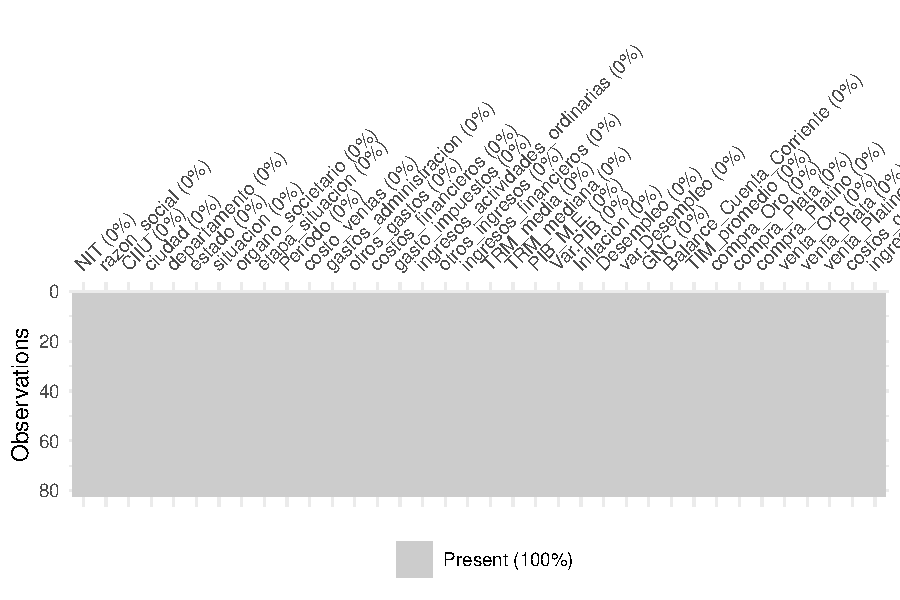
\includegraphics{index_files/figure-latex/unnamed-chunk-5-1.pdf} Esta
gráfica nos ayuda a visualizar que no hay datos perdidos en la data.

\hypertarget{capuxedtulo-4.-anuxe1lisis-descriptivo}{%
\chapter{Capítulo 4. Análisis
descriptivo}\label{capuxedtulo-4.-anuxe1lisis-descriptivo}}

A continuación se realiza un análisis descriptivo de los datos

\begin{Shaded}
\begin{Highlighting}[]
\KeywordTok{library}\NormalTok{(ggplot2)}
\KeywordTok{library}\NormalTok{(tidyr)}
\KeywordTok{library}\NormalTok{(dplyr)}

\NormalTok{datosValidar <-}\StringTok{ }\NormalTok{base_modelado }\OperatorTok\StringTok{ }\KeywordTok{group_by}\NormalTok{(NIT, razon_social) }\OperatorTok\StringTok{ }
\StringTok{  }\KeywordTok{summarise}\NormalTok{(}\DataTypeTok{total=}\KeywordTok{n}\NormalTok{())}

\NormalTok{h <-}\StringTok{ }\KeywordTok{hist}\NormalTok{(}\DataTypeTok{x =}\NormalTok{ datosValidar}\OperatorTok{$}\NormalTok{total, }\DataTypeTok{main =} \StringTok{"Cantidad de periodos por empresa"}\NormalTok{,}
          \DataTypeTok{xlab =} \StringTok{"Cantidad de periodos"}\NormalTok{, }\DataTypeTok{ylab =} \StringTok{"Empresas"}\NormalTok{, }\DataTypeTok{breaks=}\DecValTok{3}\NormalTok{)}

\KeywordTok{text}\NormalTok{(h}\OperatorTok{$}\NormalTok{mids,h}\OperatorTok{$}\NormalTok{counts,}\DataTypeTok{labels=}\NormalTok{h}\OperatorTok{$}\NormalTok{counts, }\DataTypeTok{adj=}\KeywordTok{c}\NormalTok{(}\FloatTok{0.5}\NormalTok{, }\FloatTok{-0.5}\NormalTok{))}
\end{Highlighting}
\end{Shaded}

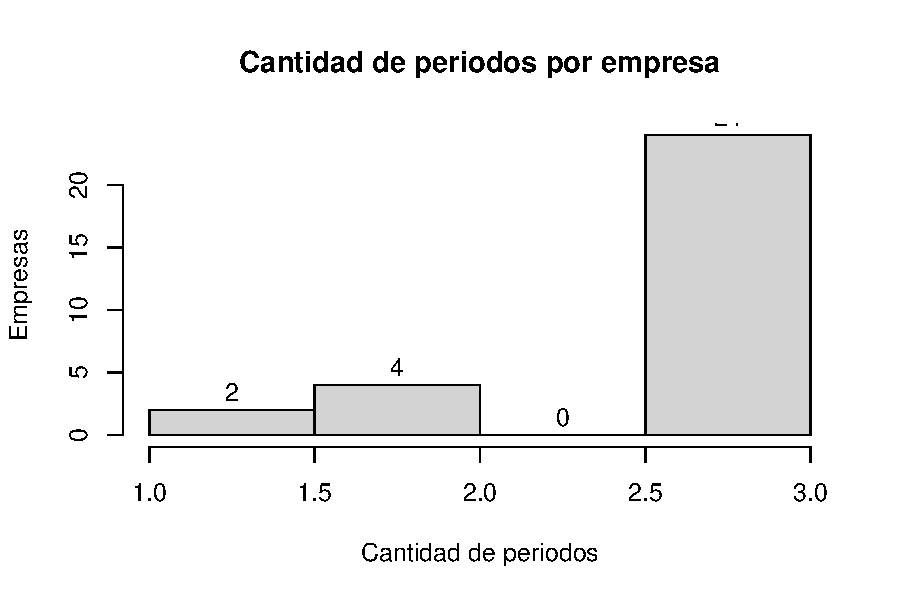
\includegraphics{index_files/figure-latex/unnamed-chunk-47-1.pdf}
Podemos observar que hay empresas que no tienen los 3 periodos, solo
trabajaremos con la empresas que tengan los periodos completos.

\begin{Shaded}
\begin{Highlighting}[]
\NormalTok{base_modelado }\OperatorTok\StringTok{ }\KeywordTok{anti_join}\NormalTok{(datosValidar }\OperatorTok\StringTok{ }\KeywordTok{filter}\NormalTok{(total }\OperatorTok{<}\StringTok{ }\DecValTok{3}\NormalTok{) , }\DataTypeTok{by=}\StringTok{"NIT"}\NormalTok{ ) }\OperatorTok\StringTok{ }
\StringTok{  }\KeywordTok{group_by}\NormalTok{(NIT, razon_social) }\OperatorTok\StringTok{ }\KeywordTok{summarise}\NormalTok{(}\DataTypeTok{total=}\KeywordTok{n}\NormalTok{()) }\OperatorTok\StringTok{ }\KeywordTok{arrange}\NormalTok{(}\KeywordTok{desc}\NormalTok{(total))}
\end{Highlighting}
\end{Shaded}

\begin{verbatim}
## # A tibble: 24 x 3
## # Groups:   NIT [24]
##    NIT       razon_social                        total
##    <chr>     <fct>                               <int>
##  1 811002172 MINERA CROESUS S.A.S                    3
##  2 830012565 ECO ORO MINERALS CORP                   3
##  3 830127076 ANGLOGOLD ASHANTI COLOMBIA S.A.         3
##  4 860507991 SANTIAGO OIL COMPANY                    3
##  5 890114642 CALDAS GOLD MARMATO S.A.S.              3
##  6 900039998 MINERALES ANDINOS DE OCCIDENTE S.A      3
##  7 900062755 MINERIA INTEGRAL DE COLOMBIA S.A.S.     3
##  8 900063262 SOCIEDAD MINERA DE SANTANDER S.A.S.     3
##  9 900084407 GRAMALOTE COLOMBIA LIMITED              3
## 10 900156833 MINERA DE COBRE QUEBRADONA  SA          3
## # ... with 14 more rows
\end{verbatim}

\begin{Shaded}
\begin{Highlighting}[]
\NormalTok{base_modelado }\OperatorTok\StringTok{ }\KeywordTok{anti_join}\NormalTok{(datosValidar }\OperatorTok\StringTok{ }\KeywordTok{filter}\NormalTok{(total }\OperatorTok{<}\StringTok{ }\DecValTok{3}\NormalTok{) , }\DataTypeTok{by=}\StringTok{"NIT"}\NormalTok{ ) ->}\StringTok{  }
\StringTok{  }\NormalTok{base_modelado}
\NormalTok{base_modelado }\OperatorTok\StringTok{ }\KeywordTok{filter}\NormalTok{(ingresos_totales }\OperatorTok{==}\StringTok{ }\DecValTok{0}\NormalTok{) }\OperatorTok\StringTok{ }\KeywordTok{count}\NormalTok{(NIT) }\OperatorTok\StringTok{ }
\StringTok{  }\KeywordTok{filter}\NormalTok{(n}\OperatorTok{==}\DecValTok{3}\NormalTok{) ->}\StringTok{ }\NormalTok{datosValidar}
\NormalTok{base_modelado }\OperatorTok\StringTok{ }\KeywordTok{anti_join}\NormalTok{(datosValidar, }\DataTypeTok{by=}\StringTok{"NIT"}\NormalTok{ )  ->}\StringTok{  }\NormalTok{base_modelado}

\NormalTok{datosValidar <-}\StringTok{ }\NormalTok{base_modelado }\OperatorTok\StringTok{ }\KeywordTok{group_by}\NormalTok{(NIT, razon_social) }\OperatorTok\StringTok{ }
\StringTok{  }\KeywordTok{summarise}\NormalTok{(}\DataTypeTok{total=}\KeywordTok{n}\NormalTok{())}

\KeywordTok{table}\NormalTok{(datosValidar}\OperatorTok{$}\NormalTok{total)}
\end{Highlighting}
\end{Shaded}

\begin{verbatim}
## 
##  3 
## 23
\end{verbatim}

Ya podemos ver que tenemos 23 empresas con los 3 periodos. Veamos los
ingresos y los costos por departamento.

\begin{Shaded}
\begin{Highlighting}[]
\NormalTok{datosValidarDepartamento <-}\StringTok{ }\NormalTok{base_modelado }\OperatorTok\StringTok{ }\KeywordTok{group_by}\NormalTok{(departamento, Periodo) }\OperatorTok\StringTok{ }
\StringTok{  }\KeywordTok{summarise}\NormalTok{(}\DataTypeTok{costo_gasto_total_dep =} \KeywordTok{sum}\NormalTok{(costos_gastos_totales) }\OperatorTok{/}\StringTok{ }\DecValTok{1000000}\NormalTok{,}
  \DataTypeTok{ingresos_totales_dep =} \KeywordTok{sum}\NormalTok{(ingresos_totales) }\OperatorTok{/}\StringTok{ }\DecValTok{1000000}\NormalTok{)}


\KeywordTok{ggplot}\NormalTok{(datosValidarDepartamento, }\KeywordTok{aes}\NormalTok{(}\DataTypeTok{x=}\NormalTok{ Periodo))}\OperatorTok{+}
\StringTok{  }\KeywordTok{geom_line}\NormalTok{(}\KeywordTok{aes}\NormalTok{(}\DataTypeTok{y =}\NormalTok{ costo_gasto_total_dep), }\DataTypeTok{color=}\StringTok{"darkred"}\NormalTok{, }\DataTypeTok{linetype=}\StringTok{"twodash"}\NormalTok{)}\OperatorTok{+}
\StringTok{  }\KeywordTok{geom_label}\NormalTok{(}\KeywordTok{aes}\NormalTok{(}\DataTypeTok{y =}\NormalTok{ costo_gasto_total_dep, }\DataTypeTok{label=}\NormalTok{costo_gasto_total_dep)) }\OperatorTok{+}\StringTok{ }
\StringTok{  }\KeywordTok{geom_line}\NormalTok{(}\KeywordTok{aes}\NormalTok{(}\DataTypeTok{y =}\NormalTok{ ingresos_totales_dep, }\DataTypeTok{label=}\StringTok{"Ingresos"}\NormalTok{), }\DataTypeTok{color =} \StringTok{"steelblue"}\NormalTok{)}\OperatorTok{+}
\StringTok{  }\KeywordTok{geom_label}\NormalTok{(}\KeywordTok{aes}\NormalTok{(}\DataTypeTok{y =}\NormalTok{ ingresos_totales_dep, }\DataTypeTok{label=}\NormalTok{ingresos_totales_dep)) }\OperatorTok{+}\StringTok{ }
\StringTok{  }\KeywordTok{facet_wrap}\NormalTok{(}\OperatorTok{~}\NormalTok{departamento, }\DataTypeTok{scales =}\StringTok{"free_y"}\NormalTok{)}
\end{Highlighting}
\end{Shaded}

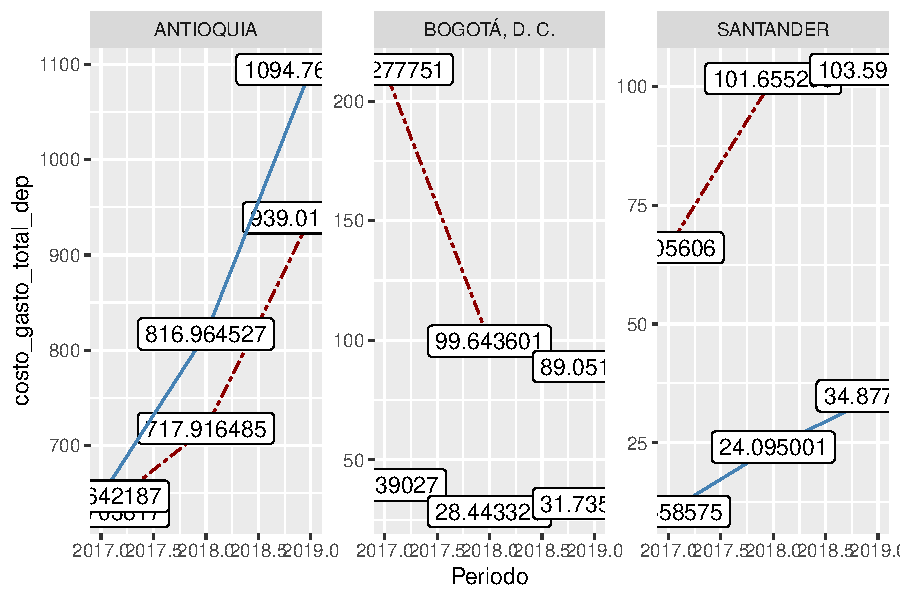
\includegraphics{index_files/figure-latex/unnamed-chunk-49-1.pdf}

\begin{Shaded}
\begin{Highlighting}[]
\NormalTok{base_modelado}\OperatorTok{$}\NormalTok{NIT=}\KeywordTok{as.factor}\NormalTok{(base_modelado}\OperatorTok{$}\NormalTok{NIT)}
\NormalTok{base_modelado}\OperatorTok{$}\NormalTok{Periodo=}\KeywordTok{as.factor}\NormalTok{(base_modelado}\OperatorTok{$}\NormalTok{Periodo)}

\NormalTok{p1=}\KeywordTok{ggplot}\NormalTok{(base_modelado, }\KeywordTok{aes}\NormalTok{(}\DataTypeTok{y=}\NormalTok{costos_gastos_totales,}\DataTypeTok{x=}\NormalTok{Periodo,}\DataTypeTok{group=}\NormalTok{NIT,}\DataTypeTok{colour=}\NormalTok{departamento))}
\NormalTok{p1}\OperatorTok{+}\KeywordTok{geom_line}\NormalTok{()}
\end{Highlighting}
\end{Shaded}

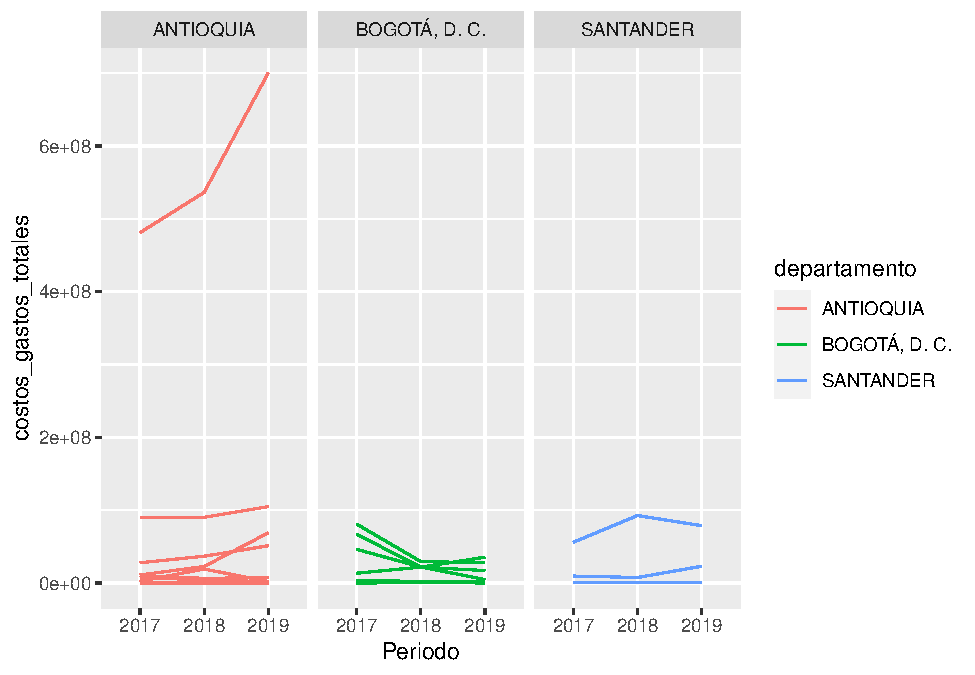
\includegraphics{index_files/figure-latex/unnamed-chunk-50-1.pdf} Se
pueden ver algunos comportamientos diferentes por departamento, sin
embargo separemos el gráfico para ver mejor:

\begin{Shaded}
\begin{Highlighting}[]
\NormalTok{p1}\OperatorTok{+}\KeywordTok{geom_line}\NormalTok{()}\OperatorTok{+}\KeywordTok{facet_grid}\NormalTok{(.}\OperatorTok{~}\NormalTok{departamento)}
\end{Highlighting}
\end{Shaded}

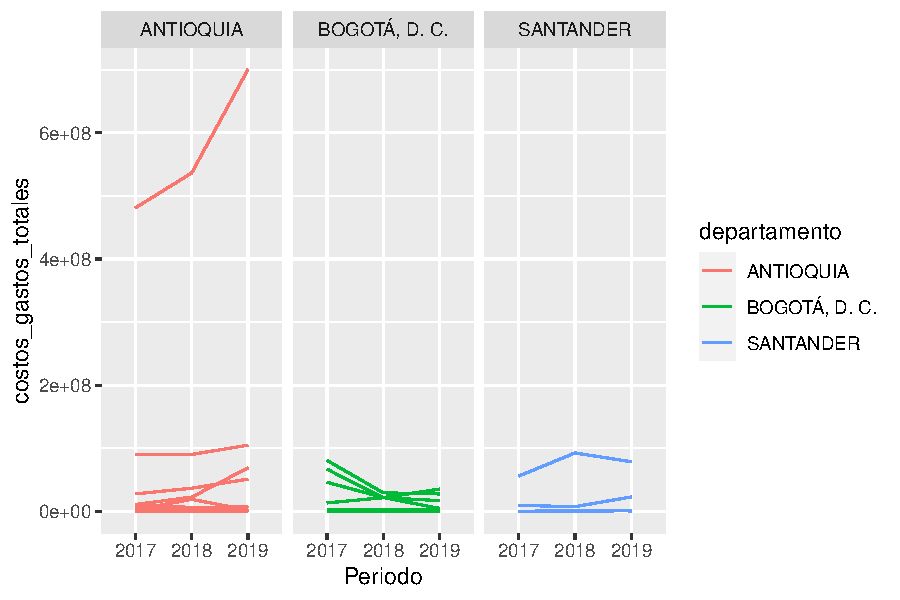
\includegraphics{index_files/figure-latex/unnamed-chunk-51-1.pdf} El
gráfico anterior nos muestra que cada empresa tiene costos/gastos
totales particulares. Adicionalmente, hay una empresa de Medellín que
tiene costos/gastos totales mas altos, comparada con las otras. Tratemos
de identificar las empresas que tienen un comportamiento más diferente a
las demás.

\begin{Shaded}
\begin{Highlighting}[]
\KeywordTok{theme_set}\NormalTok{(}\KeywordTok{theme_bw}\NormalTok{(}\DataTypeTok{base_size =} \DecValTok{8}\NormalTok{))}

\KeywordTok{qplot}\NormalTok{(NIT, costos_gastos_totales, }\DataTypeTok{facets =}\NormalTok{ . }\OperatorTok{~}\StringTok{ }\NormalTok{departamento, }
      \DataTypeTok{colour =}\NormalTok{ NIT, }\DataTypeTok{geom =} \StringTok{"boxplot"}\NormalTok{, }\DataTypeTok{data =}\NormalTok{ base_modelado)}
\end{Highlighting}
\end{Shaded}

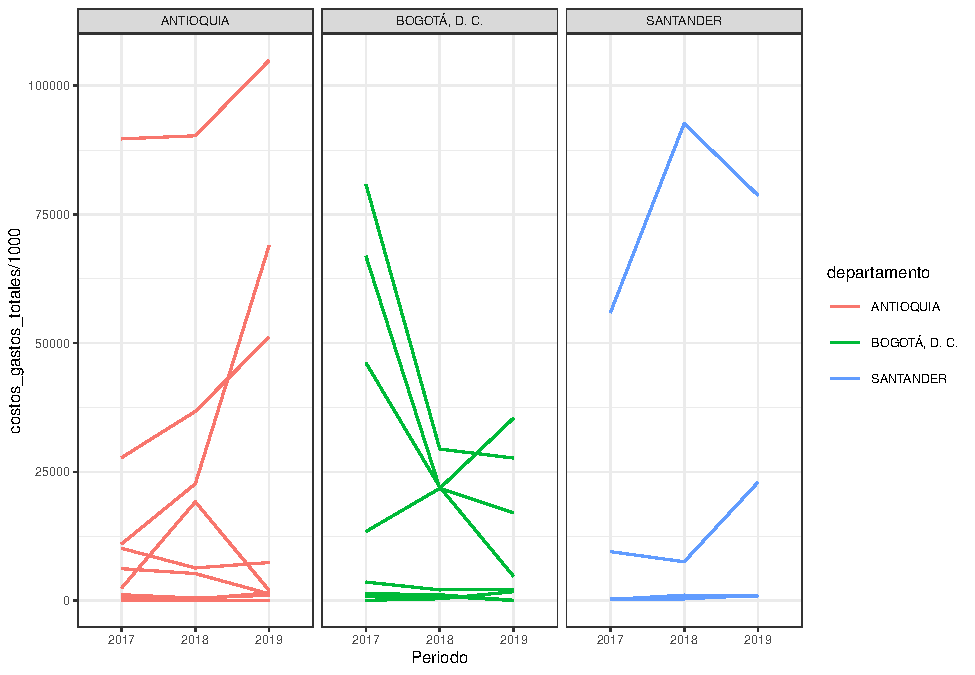
\includegraphics{index_files/figure-latex/unnamed-chunk-52-1.pdf} Al
parecer solo hay 1 empresa que tiene comportamiento de costos/gastos
totales mucho mas diferente a las demás. Realizaremos el ejercicio de
eliminar (solo para efectos visuales) la empresa que es mas diferente a
las demas.

\begin{Shaded}
\begin{Highlighting}[]
\NormalTok{datosValidar <-}\StringTok{ }\KeywordTok{filter}\NormalTok{(base_modelado, NIT}\OperatorTok{!=}\DecValTok{900306309}\NormalTok{)}
\NormalTok{p1=}\KeywordTok{ggplot}\NormalTok{(datosValidar, }\KeywordTok{aes}\NormalTok{(}\DataTypeTok{y=}\NormalTok{costos_gastos_totales}\OperatorTok{/}\DecValTok{1000}\NormalTok{,}\DataTypeTok{x=}\NormalTok{Periodo,}\DataTypeTok{group=}\NormalTok{NIT,}
                            \DataTypeTok{colour=}\NormalTok{departamento))}
\NormalTok{p1}\OperatorTok{+}\KeywordTok{geom_line}\NormalTok{()}\OperatorTok{+}\KeywordTok{facet_grid}\NormalTok{(.}\OperatorTok{~}\NormalTok{departamento)}
\end{Highlighting}
\end{Shaded}

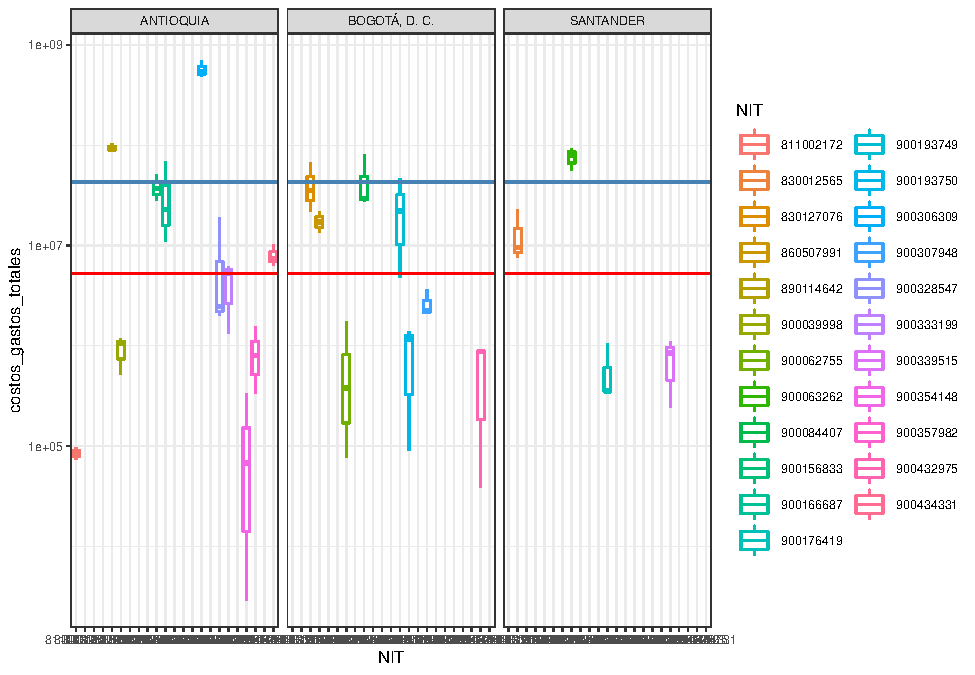
\includegraphics{index_files/figure-latex/unnamed-chunk-53-1.pdf}
Confirmamos que los costos/gastos totales son particulares de cada
empresa. Cambiemos la escala de los datos y volvamos a graficar, para
poder apreciar mejor el comportamiento de las otras empresas que tienen
costos/gastos totales mas bajos, pero con el set de empresas completo.

\begin{Shaded}
\begin{Highlighting}[]
\KeywordTok{theme_set}\NormalTok{(}\KeywordTok{theme_bw}\NormalTok{(}\DataTypeTok{base_size =} \DecValTok{8}\NormalTok{))}

\KeywordTok{qplot}\NormalTok{(NIT, costos_gastos_totales, }\DataTypeTok{facets =}\NormalTok{ . }\OperatorTok{~}\StringTok{ }\NormalTok{departamento, }
      \DataTypeTok{colour =}\NormalTok{ NIT, }\DataTypeTok{geom =} \StringTok{"boxplot"}\NormalTok{, }\DataTypeTok{data =}\NormalTok{ base_modelado) }\OperatorTok{+}
\StringTok{  }\KeywordTok{scale_y_log10}\NormalTok{() }\OperatorTok{+}\StringTok{ }
\StringTok{  }\KeywordTok{geom_hline}\NormalTok{(}\KeywordTok{aes}\NormalTok{(}\DataTypeTok{yintercept =} \KeywordTok{mean}\NormalTok{(costos_gastos_totales)), }\DataTypeTok{color =} \StringTok{"steelblue"}\NormalTok{) }\OperatorTok{+}
\StringTok{  }
\StringTok{  }\KeywordTok{geom_hline}\NormalTok{(}\KeywordTok{aes}\NormalTok{(}\DataTypeTok{yintercept =} \KeywordTok{median}\NormalTok{(costos_gastos_totales)), }\DataTypeTok{color =} \StringTok{"red"}\NormalTok{)}
\end{Highlighting}
\end{Shaded}

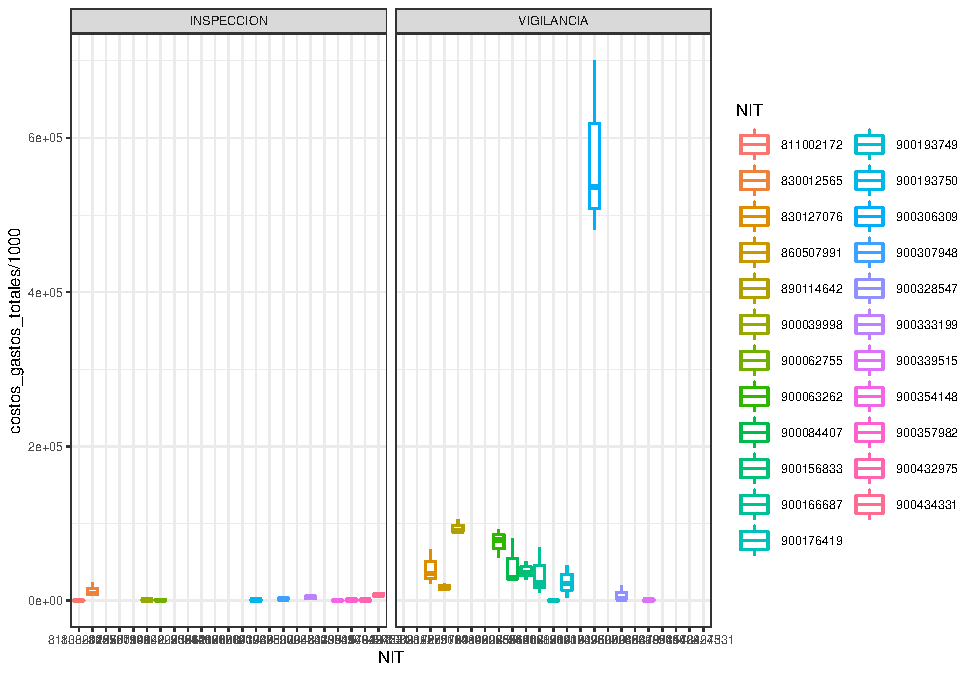
\includegraphics{index_files/figure-latex/unnamed-chunk-54-1.pdf} Ahora
podemos ver mejor que cada empresa tiene unos costos/gastos totales
particulares, así como costos promedio diferentes. Además, encontramos
que solamente hay 5 empresas que tienen un comportamiento general en sus
costos/gastos totales. Ahora revisemos los costos/gastos totales con el
estado.

\begin{Shaded}
\begin{Highlighting}[]
\KeywordTok{theme_set}\NormalTok{(}\KeywordTok{theme_bw}\NormalTok{(}\DataTypeTok{base_size =} \DecValTok{8}\NormalTok{))}

\KeywordTok{qplot}\NormalTok{(NIT, costos_gastos_totales}\OperatorTok{/}\DecValTok{1000}\NormalTok{, }\DataTypeTok{facets =}\NormalTok{ . }\OperatorTok{~}\StringTok{ }\NormalTok{estado, }
      \DataTypeTok{colour =}\NormalTok{ NIT, }\DataTypeTok{geom =} \StringTok{"boxplot"}\NormalTok{, }\DataTypeTok{data =}\NormalTok{ base_modelado) }
\end{Highlighting}
\end{Shaded}

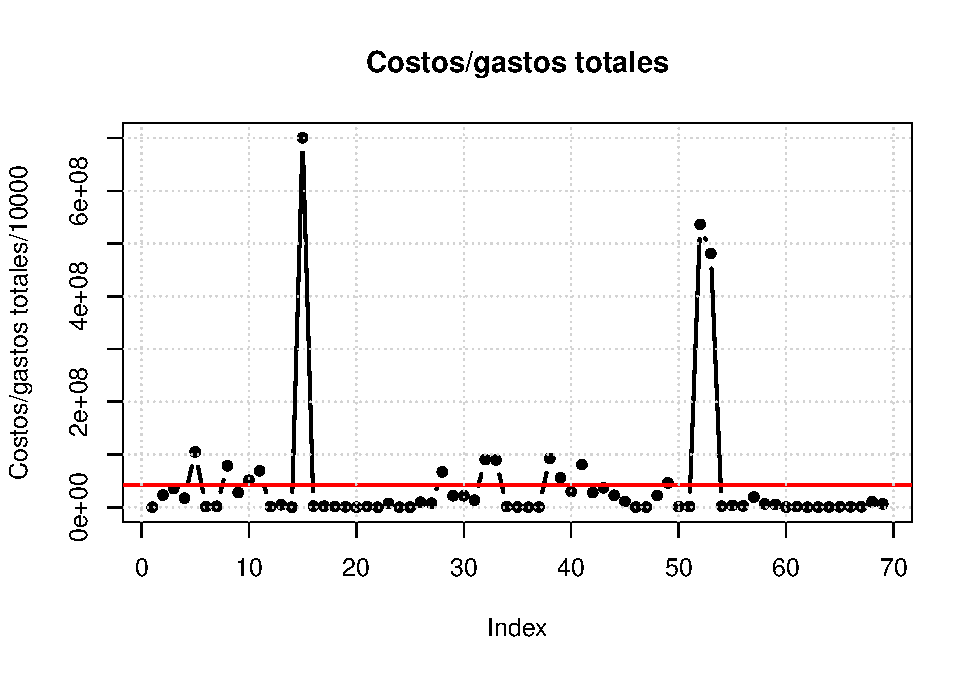
\includegraphics{index_files/figure-latex/unnamed-chunk-55-1.pdf}
Podemos ver que las empresas con estado inspección presentan
costos/gastos totales menores que las empresas con estado vigilancia.
Veamos ahora la dispersion de nuestra variable objetivo.

\begin{Shaded}
\begin{Highlighting}[]
\KeywordTok{plot}\NormalTok{(base_modelado}\OperatorTok{$}\NormalTok{costos_gastos_totales, }\DataTypeTok{main=}\StringTok{"Costos/gastos totales"}\NormalTok{,}
    \DataTypeTok{type=}\StringTok{"b"}\NormalTok{, }\DataTypeTok{ylab=}\StringTok{"Costos/gastos totales/10000"}\NormalTok{, }\DataTypeTok{pch=} \DecValTok{20}\NormalTok{, }\DataTypeTok{lwd=}\DecValTok{2}\NormalTok{)}
\KeywordTok{abline}\NormalTok{(}\DataTypeTok{h=}\KeywordTok{mean}\NormalTok{(base_modelado}\OperatorTok{$}\NormalTok{costos_gastos_totales), }\DataTypeTok{lwd=}\DecValTok{2}\NormalTok{, }\DataTypeTok{col=} \StringTok{"red"}\NormalTok{)}
\KeywordTok{grid}\NormalTok{()}
\end{Highlighting}
\end{Shaded}

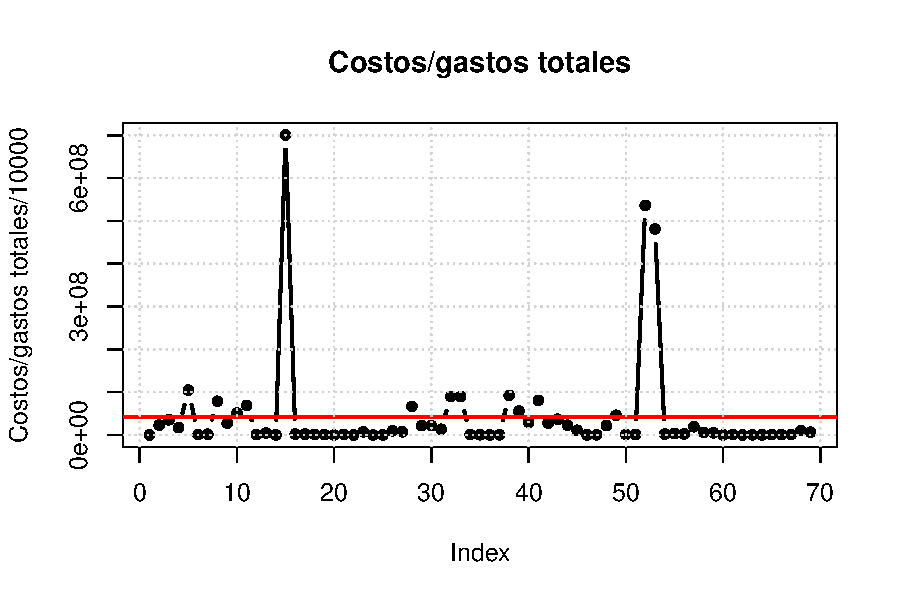
\includegraphics{index_files/figure-latex/unnamed-chunk-56-1.pdf} Con
esto confirmamos que la dispersion de los costos/gastos totales no tiene
un comportamiento general.

\hypertarget{estandarizaciuxf3n-de-variables}{%
\section{Estandarización de
variables}\label{estandarizaciuxf3n-de-variables}}

A continuación se realiza un reescalamiento de las variables para que
sean comparables y así apuntarle a mejorar la calidad de los modelos

\begin{Shaded}
\begin{Highlighting}[]
\KeywordTok{library}\NormalTok{(scales)}
\KeywordTok{library}\NormalTok{(kableExtra)}
\KeywordTok{library}\NormalTok{(tibble)}
\NormalTok{base.escalada<-}\StringTok{ }\KeywordTok{scale}\NormalTok{(base_modelado[,}\KeywordTok{c}\NormalTok{(}\DecValTok{11}\NormalTok{,}\DecValTok{12}\NormalTok{, }\DecValTok{13}\NormalTok{,}\DecValTok{14}\NormalTok{,}\DecValTok{15}\NormalTok{,}\DecValTok{16}\NormalTok{,}\DecValTok{17}\NormalTok{,}\DecValTok{18}\NormalTok{,}\DecValTok{19}\NormalTok{,}\DecValTok{20}\NormalTok{,}\DecValTok{21}\NormalTok{,}\DecValTok{22}\NormalTok{,}\DecValTok{23}\NormalTok{,}
                    \DecValTok{24}\NormalTok{,}\DecValTok{25}\NormalTok{,}\DecValTok{26}\NormalTok{,}\DecValTok{27}\NormalTok{,}\DecValTok{28}\NormalTok{,}\DecValTok{29}\NormalTok{,}\DecValTok{30}\NormalTok{,}\DecValTok{31}\NormalTok{,}\DecValTok{32}\NormalTok{,}\DecValTok{33}\NormalTok{,}\DecValTok{34}\NormalTok{,}\DecValTok{35}\NormalTok{,}\DecValTok{36}\NormalTok{)],}\DataTypeTok{center=}\NormalTok{T,}\DataTypeTok{scale=}\NormalTok{T)}
\NormalTok{base.escalada<-}\StringTok{ }\KeywordTok{as.data.frame}\NormalTok{(base.escalada)}
\NormalTok{base.escalada<-}\StringTok{ }\KeywordTok{rownames_to_column}\NormalTok{(base.escalada)}
\NormalTok{tmp <-}\StringTok{ }\KeywordTok{rownames_to_column}\NormalTok{(base_modelado }\OperatorTok\StringTok{ }\KeywordTok{select}\NormalTok{(}\KeywordTok{c}\NormalTok{(}\StringTok{"NIT"}\NormalTok{, }\StringTok{"razon_social"}\NormalTok{, }
  \StringTok{"CIIU"}\NormalTok{, }\StringTok{"ciudad"}\NormalTok{,}\StringTok{"departamento"}\NormalTok{, }\StringTok{"estado"}\NormalTok{, }\StringTok{"situacion"}\NormalTok{, }\StringTok{"organo_societario"}\NormalTok{,}
  \StringTok{"etapa_situacion"}\NormalTok{, }\StringTok{"Periodo"}\NormalTok{)))}
\NormalTok{base_modelado <-}\StringTok{ }\NormalTok{tmp }\OperatorTok\StringTok{ }\KeywordTok{left_join}\NormalTok{(base.escalada, }\DataTypeTok{by=}\StringTok{"rowname"}\NormalTok{) }\OperatorTok\StringTok{ }
\StringTok{  }\KeywordTok{select}\NormalTok{(}\OperatorTok{-}\KeywordTok{c}\NormalTok{(}\StringTok{"rowname"}\NormalTok{))}
\end{Highlighting}
\end{Shaded}

\hypertarget{capuxedtulo-5.-correlaciones}{%
\chapter{Capítulo 5. Correlaciones}\label{capuxedtulo-5.-correlaciones}}

En este capítulo realizaremos un análisis de las correlaciones entre las
variables que nos ayudarán a decidir que variables pueden ser las
mejores candidatas para nuestro modelo.

La base de datos que utilizaremos es \texttt{base\_modelado} la misma
que visualizamos en la página 15

\begin{Shaded}
\begin{Highlighting}[]
\KeywordTok{head}\NormalTok{(base_modelado)}
\end{Highlighting}
\end{Shaded}

\begin{verbatim}
##         NIT                       razon_social  CIIU       ciudad  departamento
## 1 811002172               MINERA CROESUS S.A.S B0722     MEDELLÍN     ANTIOQUIA
## 2 830012565              ECO ORO MINERALS CORP B0722  BUCARAMANGA     SANTANDER
## 3 830127076    ANGLOGOLD ASHANTI COLOMBIA S.A. B0722 BOGOTÁ, D.C. BOGOTÁ, D. C.
## 4 860507991               SANTIAGO OIL COMPANY B0722 BOGOTÁ, D.C. BOGOTÁ, D. C.
## 5 890114642         CALDAS GOLD MARMATO S.A.S. B0722     MEDELLÍN     ANTIOQUIA
## 6 900039998 MINERALES ANDINOS DE OCCIDENTE S.A B0722     MEDELLÍN     ANTIOQUIA
##       estado situacion             organo_societario etapa_situacion Periodo
## 1 INSPECCION    ACTIVA ACTIVIDAD ECONOMICA DIFERENTE          ACTIVA    2019
## 2 INSPECCION    ACTIVA ACTIVIDAD ECONOMICA DIFERENTE          ACTIVA    2019
## 3 VIGILANCIA    ACTIVA ACTIVIDAD ECONOMICA DIFERENTE          ACTIVA    2019
## 4 VIGILANCIA    ACTIVA ACTIVIDAD ECONOMICA DIFERENTE          ACTIVA    2019
## 5 VIGILANCIA    ACTIVA ACTIVIDAD ECONOMICA DIFERENTE          ACTIVA    2019
## 6 INSPECCION    ACTIVA ACTIVIDAD ECONOMICA DIFERENTE          ACTIVA    2019
##   costo_ventas gastos_administracion otros_gastos costos_financieros
## 1  -0.33867199            -0.4074151   -0.4014073        -0.01766357
## 2  -0.33867199            -0.1245786    1.7804892        -0.41681165
## 3   0.14621874            -0.4096184   -0.4014073        -0.11939539
## 4  -0.04073369            -0.3719525   -0.3443104         0.18991196
## 5   0.96663837            -0.3124819   -0.3166147        -0.12092215
## 6  -0.33867199            -0.4096184   -0.2576751         0.45676213
##   gasto_impuestos ingresos_actividades_ordinarias otros_ingresos
## 1     -0.22397057                     -0.23958426    0.005953155
## 2     -0.22262585                     -0.23958426   -0.210004581
## 3     -0.22477997                     -0.23958426   -0.508192736
## 4     -0.48682468                     -0.06443343   -0.363463888
## 5      0.05505802                      0.51657397    0.383638219
## 6     -0.22467562                     -0.23958426   -0.508192736
##   ingresos_financieros TRM_media TRM_mediana  PIB_M.E.   Var.PIB Inflacion
## 1           -0.3515285    1.4038     1.39604 -1.385842 0.2183709 0.2877006
## 2           -0.3515285    1.4038     1.39604 -1.385842 0.2183709 0.2877006
## 3           -0.3515285    1.4038     1.39604 -1.385842 0.2183709 0.2877006
## 4           -0.1320566    1.4038     1.39604 -1.385842 0.2183709 0.2877006
## 5            0.4181071    1.4038     1.39604 -1.385842 0.2183709 0.2877006
## 6           -0.3515285    1.4038     1.39604 -1.385842 0.2183709 0.2877006
##   Desempleo var.Desempleo      GNC Balance_Cuenta_Corriente TIM_promedio
## 1  1.354199      1.380845 1.250959               -0.1990925   -0.7586531
## 2  1.354199      1.380845 1.250959               -0.1990925   -0.7586531
## 3  1.354199      1.380845 1.250959               -0.1990925   -0.7586531
## 4  1.354199      1.380845 1.250959               -0.1990925   -0.7586531
## 5  1.354199      1.380845 1.250959               -0.1990925   -0.7586531
## 6  1.354199      1.380845 1.250959               -0.1990925   -0.7586531
##   compra_Oro compra_Plata compra_Platino venta_Oro venta_Plata venta_Platino
## 1   1.403075     1.151478      0.8708067  1.403075     1.15238     0.8708068
## 2   1.403075     1.151478      0.8708067  1.403075     1.15238     0.8708068
## 3   1.403075     1.151478      0.8708067  1.403075     1.15238     0.8708068
## 4   1.403075     1.151478      0.8708067  1.403075     1.15238     0.8708068
## 5   1.403075     1.151478      0.8708067  1.403075     1.15238     0.8708068
## 6   1.403075     1.151478      0.8708067  1.403075     1.15238     0.8708068
##   costos_gastos_totales ingresos_totales
## 1           -0.36104643      -0.24581787
## 2           -0.16782320      -0.24842906
## 3           -0.06283635      -0.25203452
## 4           -0.21786041      -0.07148885
## 5            0.52255596       0.52606828
## 6           -0.35276218      -0.25203452
\end{verbatim}

Para el análisis de correlaciones, se toman las variables
macroeconómicas (PIB, Inflación, Desempleo, GNC, Balance de cuenta
corriente y TRM), compra y venta de metales preciosos y se compara con
la variable objetivo.

\hypertarget{calcular-el-coeficiente-de-correlaciuxf3n}{%
\subsection{Calcular el coeficiente de
correlación}\label{calcular-el-coeficiente-de-correlaciuxf3n}}

Este comando calcula la matriz de correlación:

\begin{verbatim}
##                          TRM_media TRM_mediana PIB_M.E. Var.PIB Inflacion
## TRM_media                     1.00        0.99    -0.99    0.14      0.19
## TRM_mediana                   0.99        1.00    -0.96    0.26      0.31
## PIB_M.E.                     -0.99       -0.96     1.00    0.00     -0.05
## Var.PIB                       0.14        0.26     0.00    1.00      1.00
## Inflacion                     0.19        0.31    -0.05    1.00      1.00
## Desempleo                     0.97        0.93    -0.99   -0.11     -0.06
## var.Desempleo                 0.99        0.96    -1.00   -0.03      0.02
## GNC                           0.90        0.84    -0.95   -0.31     -0.26
## Balance_Cuenta_Corriente     -0.13       -0.25    -0.02   -1.00     -1.00
## TIM_promedio                 -0.55       -0.45     0.67    0.75      0.71
## compra_Oro                    1.00        0.99    -0.99    0.12      0.17
## compra_Plata                  0.81        0.88    -0.72    0.69      0.73
## compra_Platino                0.61        0.70    -0.49    0.87      0.89
## venta_Oro                     1.00        0.99    -0.99    0.12      0.17
## venta_Plata                   0.81        0.88    -0.72    0.69      0.73
## venta_Platino                 0.61        0.70    -0.49    0.87      0.89
## Var.objetivo                  0.04        0.04    -0.04    0.00      0.01
##                          Desempleo var.Desempleo   GNC Balance_Cuenta_Corriente
## TRM_media                     0.97          0.99  0.90                    -0.13
## TRM_mediana                   0.93          0.96  0.84                    -0.25
## PIB_M.E.                     -0.99         -1.00 -0.95                    -0.02
## Var.PIB                      -0.11         -0.03 -0.31                    -1.00
## Inflacion                    -0.06          0.02 -0.26                    -1.00
## Desempleo                     1.00          1.00  0.98                     0.12
## var.Desempleo                 1.00          1.00  0.96                     0.04
## GNC                           0.98          0.96  1.00                     0.32
## Balance_Cuenta_Corriente      0.12          0.04  0.32                     1.00
## TIM_promedio                 -0.74         -0.68 -0.86                    -0.76
## compra_Oro                    0.97          0.99  0.91                    -0.11
## compra_Plata                  0.64          0.70  0.47                    -0.68
## compra_Platino                0.39          0.47  0.20                    -0.86
## venta_Oro                     0.97          0.99  0.91                    -0.11
## venta_Plata                   0.64          0.70  0.47                    -0.68
## venta_Platino                 0.39          0.47  0.20                    -0.86
## Var.objetivo                  0.04          0.04  0.03                     0.00
##                          TIM_promedio compra_Oro compra_Plata compra_Platino
## TRM_media                       -0.55       1.00         0.81           0.61
## TRM_mediana                     -0.45       0.99         0.88           0.70
## PIB_M.E.                         0.67      -0.99        -0.72          -0.49
## Var.PIB                          0.75       0.12         0.69           0.87
## Inflacion                        0.71       0.17         0.73           0.89
## Desempleo                       -0.74       0.97         0.64           0.39
## var.Desempleo                   -0.68       0.99         0.70           0.47
## GNC                             -0.86       0.91         0.47           0.20
## Balance_Cuenta_Corriente        -0.76      -0.11        -0.68          -0.86
## TIM_promedio                     1.00      -0.57         0.04           0.32
## compra_Oro                      -0.57       1.00         0.80           0.59
## compra_Plata                     0.04       0.80         1.00           0.96
## compra_Platino                   0.32       0.59         0.96           1.00
## venta_Oro                       -0.57       1.00         0.80           0.59
## venta_Plata                      0.04       0.80         1.00           0.96
## venta_Platino                    0.32       0.59         0.96           1.00
## Var.objetivo                    -0.02       0.04         0.03           0.02
##                          venta_Oro venta_Plata venta_Platino Var.objetivo
## TRM_media                     1.00        0.81          0.61         0.04
## TRM_mediana                   0.99        0.88          0.70         0.04
## PIB_M.E.                     -0.99       -0.72         -0.49        -0.04
## Var.PIB                       0.12        0.69          0.87         0.00
## Inflacion                     0.17        0.73          0.89         0.01
## Desempleo                     0.97        0.64          0.39         0.04
## var.Desempleo                 0.99        0.70          0.47         0.04
## GNC                           0.91        0.47          0.20         0.03
## Balance_Cuenta_Corriente     -0.11       -0.68         -0.86         0.00
## TIM_promedio                 -0.57        0.04          0.32        -0.02
## compra_Oro                    1.00        0.80          0.59         0.04
## compra_Plata                  0.80        1.00          0.96         0.03
## compra_Platino                0.59        0.96          1.00         0.02
## venta_Oro                     1.00        0.80          0.59         0.04
## venta_Plata                   0.80        1.00          0.96         0.03
## venta_Platino                 0.59        0.96          1.00         0.02
## Var.objetivo                  0.04        0.03          0.02         1.00
\end{verbatim}

Con el resultado de la correlación, podemos interpretar que las
variables macroeconomicas, compra y venta de metales preciosos no
explican la variable objetivo, ya que el nivel de significancia es
cercano a cero. Es decir, no encontramos una ascociación entre estas
variables y la variable objetivo, que nos ayude a predecir o explicar el
comportamiento de los costos y gastos totales de las empresas del sector
``extracción de oro y otros metales preciosos''.

\hypertarget{visualizar-matriz-de-correlaciuxf3n}{%
\subsection{Visualizar matriz de
correlación}\label{visualizar-matriz-de-correlaciuxf3n}}

Utilizaremos el comando corrplot para visualizar la matriz de
correlaciones. Lo primero es calcular la matriz, guardarla en un objeto
y luego graficarla. En este caso vamos a graficar los coeficientes
resultantes.

\begin{Shaded}
\begin{Highlighting}[]
\NormalTok{correlacion<-}\KeywordTok{round}\NormalTok{(}\KeywordTok{cor}\NormalTok{(base), }\DecValTok{1}\NormalTok{)}

\KeywordTok{corrplot}\NormalTok{(correlacion, }\DataTypeTok{method=}\StringTok{"number"}\NormalTok{, }\DataTypeTok{type=}\StringTok{"upper"}\NormalTok{)}
\end{Highlighting}
\end{Shaded}

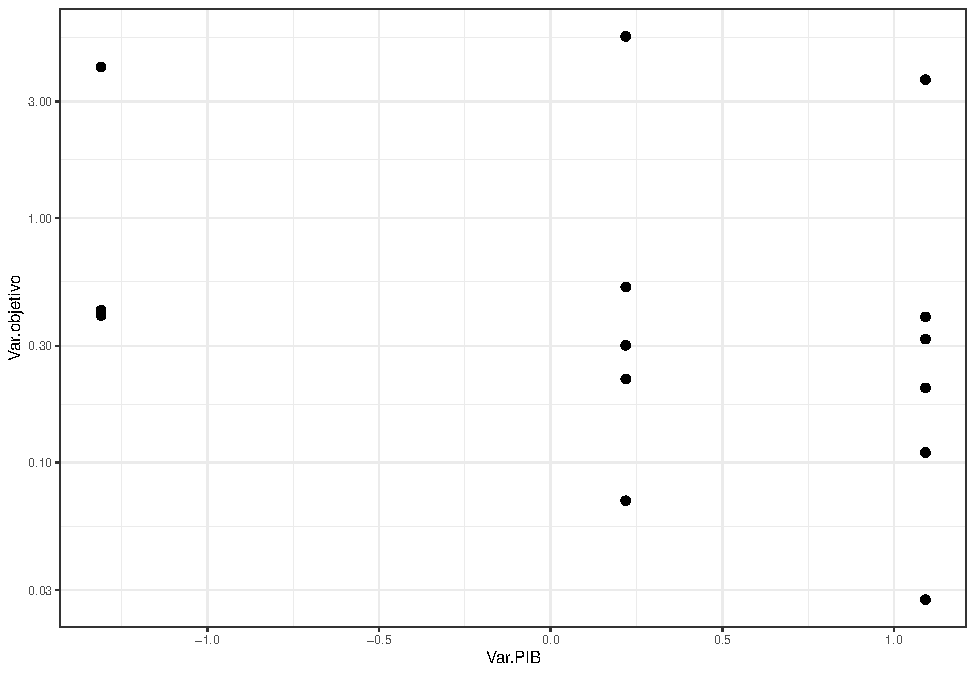
\includegraphics{index_files/figure-latex/unnamed-chunk-61-1.pdf} Se
realizó el análisis de correlación con el estadístico de Pearson, con
las variables originales y estandarizadas, con el fin de evidenciar las
variables explicativas de la variable objetivo construida, encontrando
como resultado la no significancia para explicar el comportamiento de
los costos y gastos del sector que estamos estudiando.

A continuación se grafican los datos de la Variable objetivo (costos y
gastos totales) con respecto a var.PIB (Variación del PIB)

\begin{Shaded}
\begin{Highlighting}[]
\KeywordTok{ggplot}\NormalTok{(base, }\KeywordTok{aes}\NormalTok{(}\DataTypeTok{x=}\NormalTok{Var.PIB, }\DataTypeTok{y=}\NormalTok{Var.objetivo)) }\OperatorTok{+}\KeywordTok{geom_point}\NormalTok{()}\OperatorTok{+}\KeywordTok{scale_y_log10}\NormalTok{()}
\end{Highlighting}
\end{Shaded}

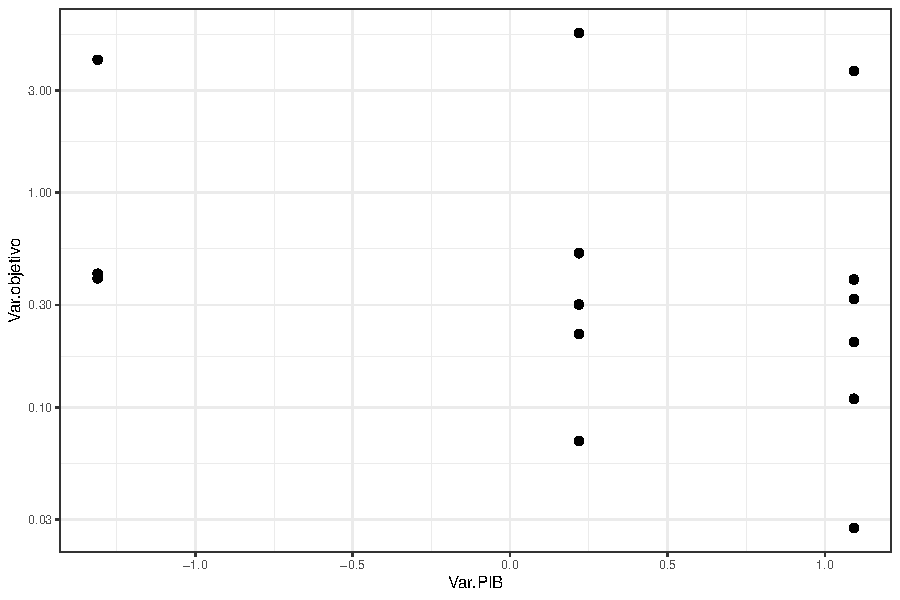
\includegraphics{index_files/figure-latex/unnamed-chunk-62-1.pdf}
Podemos apreciar que no se presenta un comportamiento lineal entre las
variables, por lo tanto la variable PIB no es una buena candidata para
utilizar en nuestro modelo. De forma general encontramos que las
macroeconómicas no explican la variable objetivo. Por tal motivo se
decide no trabajar con las variables macroeconomicas venta y compra de
metales preciosos en los modelos.

Sin embargo adicionamos a nuestra base de datos estas variables
económicas que servirán de insumo para la fase de modelado.

\begin{Shaded}
\begin{Highlighting}[]
\NormalTok{base_modelado }\OperatorTok\StringTok{ }\KeywordTok{select}\NormalTok{(departamento, estado, Periodo, costos_gastos_totales,}
\NormalTok{  ciudad, ingresos_totales, NIT, razon_social,otros_ingresos ,}
\NormalTok{  ingresos_financieros, compra_Oro, compra_Plata, compra_Platino, venta_Oro, }
\NormalTok{  venta_Plata, venta_Platino) ->}\StringTok{ }\NormalTok{base_modelo_lineal}

\CommentTok{#definir variable de tamaño de la empresa}
\NormalTok{bussiness_size <-}\StringTok{ }\KeywordTok{cut}\NormalTok{(base_modelo_lineal}\OperatorTok{$}\NormalTok{costos_gastos_totales, }\DataTypeTok{breaks=}\DecValTok{4}\NormalTok{)}
\KeywordTok{levels}\NormalTok{(bussiness_size) <-}\StringTok{ }\KeywordTok{list}\NormalTok{(}\DataTypeTok{small =} \StringTok{"(-0.377,0.349]"}\NormalTok{, }
                               \DataTypeTok{medium =} \StringTok{"(0.349,1.07]"}\NormalTok{, }
                               \DataTypeTok{big =} \StringTok{"(1.07,1.8]"}\NormalTok{, }
                               \DataTypeTok{very_big=}\StringTok{"(1.8,2.52]"}\NormalTok{)}
\NormalTok{base_modelo_lineal[}\StringTok{'tamano_empresa'}\NormalTok{] <-}\StringTok{ }\NormalTok{bussiness_size}
\NormalTok{base_modelo_lineal }\OperatorTok\StringTok{ }\KeywordTok{filter}\NormalTok{(NIT }\OperatorTok{!=}\StringTok{ }\DecValTok{900306309}\NormalTok{) ->}\StringTok{ }\NormalTok{base_modelo_lineal}
\KeywordTok{head}\NormalTok{(base_modelo_lineal)}
\end{Highlighting}
\end{Shaded}

\begin{verbatim}
##    departamento     estado Periodo costos_gastos_totales       ciudad
## 1     ANTIOQUIA INSPECCION    2019           -0.36104643     MEDELLÍN
## 2     SANTANDER INSPECCION    2019           -0.16782320  BUCARAMANGA
## 3 BOGOTÁ, D. C. VIGILANCIA    2019           -0.06283635 BOGOTÁ, D.C.
## 4 BOGOTÁ, D. C. VIGILANCIA    2019           -0.21786041 BOGOTÁ, D.C.
## 5     ANTIOQUIA VIGILANCIA    2019            0.52255596     MEDELLÍN
## 6     ANTIOQUIA INSPECCION    2019           -0.35276218     MEDELLÍN
##   ingresos_totales       NIT                       razon_social otros_ingresos
## 1      -0.24581787 811002172               MINERA CROESUS S.A.S    0.005953155
## 2      -0.24842906 830012565              ECO ORO MINERALS CORP   -0.210004581
## 3      -0.25203452 830127076    ANGLOGOLD ASHANTI COLOMBIA S.A.   -0.508192736
## 4      -0.07148885 860507991               SANTIAGO OIL COMPANY   -0.363463888
## 5       0.52606828 890114642         CALDAS GOLD MARMATO S.A.S.    0.383638219
## 6      -0.25203452 900039998 MINERALES ANDINOS DE OCCIDENTE S.A   -0.508192736
##   ingresos_financieros compra_Oro compra_Plata compra_Platino venta_Oro
## 1           -0.3515285   1.403075     1.151478      0.8708067  1.403075
## 2           -0.3515285   1.403075     1.151478      0.8708067  1.403075
## 3           -0.3515285   1.403075     1.151478      0.8708067  1.403075
## 4           -0.1320566   1.403075     1.151478      0.8708067  1.403075
## 5            0.4181071   1.403075     1.151478      0.8708067  1.403075
## 6           -0.3515285   1.403075     1.151478      0.8708067  1.403075
##   venta_Plata venta_Platino tamano_empresa
## 1     1.15238     0.8708068           <NA>
## 2     1.15238     0.8708068           <NA>
## 3     1.15238     0.8708068           <NA>
## 4     1.15238     0.8708068           <NA>
## 5     1.15238     0.8708068           <NA>
## 6     1.15238     0.8708068           <NA>
\end{verbatim}

\hypertarget{capuxedtulo-6.-aplicaciuxf3n-de-modelo}{%
\chapter{Capítulo 6. Aplicación de
modelo}\label{capuxedtulo-6.-aplicaciuxf3n-de-modelo}}

\hypertarget{modelo-regresiuxf3n-lineal---con-todas-las-variables-de-compra-y-venta-de-oro}{%
\subsection{6.1. Modelo regresión Lineal - con todas las variables de
compra y venta de
oro}\label{modelo-regresiuxf3n-lineal---con-todas-las-variables-de-compra-y-venta-de-oro}}

En este modelo se intenta explicar los costos y gastos en función de las
variables de compra y venta de metales preciosos.

\begin{Shaded}
\begin{Highlighting}[]
\KeywordTok{library}\NormalTok{(broom)}

\NormalTok{mod1 <-}\StringTok{ }\KeywordTok{lm}\NormalTok{(costos_gastos_totales }\OperatorTok{~}\StringTok{  }\NormalTok{compra_Oro }\OperatorTok{+}\StringTok{ }\NormalTok{compra_Plata }\OperatorTok{+}\StringTok{ }\NormalTok{compra_Platino }\OperatorTok{+}\StringTok{ }
\StringTok{        }\NormalTok{venta_Oro }\OperatorTok{+}\StringTok{ }\NormalTok{venta_Plata }\OperatorTok{+}\StringTok{ }\NormalTok{venta_Platino }\OperatorTok{+}\StringTok{ }\NormalTok{ingresos_totales, }
        \DataTypeTok{data=}\NormalTok{ base_modelo_lineal) }
\KeywordTok{anova}\NormalTok{(mod1)}
\end{Highlighting}
\end{Shaded}

\begin{verbatim}
## Analysis of Variance Table
## 
## Response: costos_gastos_totales
##                  Df  Sum Sq Mean Sq F value    Pr(>F)    
## compra_Oro        1 0.00121 0.00121  0.0379    0.8462    
## compra_Plata      1 0.00359 0.00359  0.1122    0.7388    
## ingresos_totales  1 1.64429 1.64429 51.3861 1.098e-09 ***
## Residuals        62 1.98392 0.03200                      
## ---
## Signif. codes:  0 '***' 0.001 '**' 0.01 '*' 0.05 '.' 0.1 ' ' 1
\end{verbatim}

Calculamos el resumen del modelo 1:

\begin{Shaded}
\begin{Highlighting}[]
\KeywordTok{summary}\NormalTok{(mod1)}
\end{Highlighting}
\end{Shaded}

\begin{verbatim}
## 
## Call:
## lm(formula = costos_gastos_totales ~ compra_Oro + compra_Plata + 
##     compra_Platino + venta_Oro + venta_Plata + venta_Platino + 
##     ingresos_totales, data = base_modelo_lineal)
## 
## Residuals:
##      Min       1Q   Median       3Q      Max 
## -0.19751 -0.10238 -0.08597  0.06201  0.56114 
## 
## Coefficients: (4 not defined because of singularities)
##                  Estimate Std. Error t value Pr(>|t|)    
## (Intercept)       0.02387    0.03855   0.619    0.538    
## compra_Oro       -0.01201    0.03696  -0.325    0.746    
## compra_Plata      0.01249    0.03695   0.338    0.736    
## compra_Platino         NA         NA      NA       NA    
## venta_Oro              NA         NA      NA       NA    
## venta_Plata            NA         NA      NA       NA    
## venta_Platino          NA         NA      NA       NA    
## ingresos_totales  1.11327    0.15530   7.168  1.1e-09 ***
## ---
## Signif. codes:  0 '***' 0.001 '**' 0.01 '*' 0.05 '.' 0.1 ' ' 1
## 
## Residual standard error: 0.1789 on 62 degrees of freedom
## Multiple R-squared:  0.4539, Adjusted R-squared:  0.4275 
## F-statistic: 17.18 on 3 and 62 DF,  p-value: 3.124e-08
\end{verbatim}

\begin{Shaded}
\begin{Highlighting}[]
\NormalTok{a <-}\StringTok{ }\KeywordTok{augment}\NormalTok{(mod1)}
\KeywordTok{ggplot}\NormalTok{(a, }\KeywordTok{aes}\NormalTok{(}\DataTypeTok{x=}\DecValTok{1}\OperatorTok{:}\KeywordTok{length}\NormalTok{(.resid), }\DataTypeTok{y=}\NormalTok{.resid))}\OperatorTok{+}
\StringTok{  }\KeywordTok{geom_point}\NormalTok{() }\OperatorTok{+}\StringTok{ }
\StringTok{  }\KeywordTok{geom_hline}\NormalTok{(}\DataTypeTok{yintercept =} \DecValTok{0}\NormalTok{, }\DataTypeTok{lwd=}\DecValTok{2}\NormalTok{, }\DataTypeTok{col=} \StringTok{"red"}\NormalTok{)}
\end{Highlighting}
\end{Shaded}

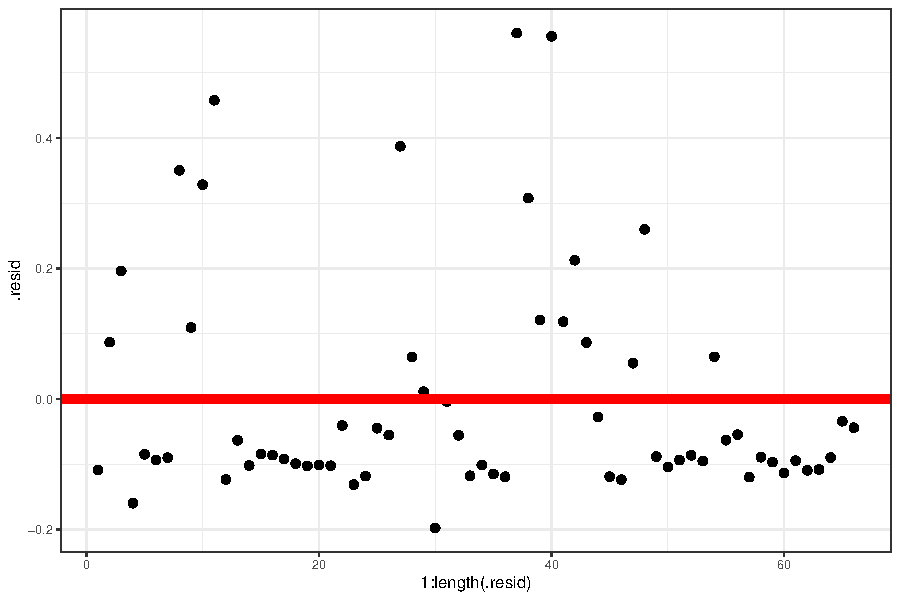
\includegraphics{index_files/figure-latex/unnamed-chunk-12-1.pdf}

Evaluación de los modelos: AIC, BIC y R2.

El AIC NO es una prueba de hipótesis sobre el ajuste de un modelo, sino
más bien un criterio paramétrico comparativo entre modelos y representa
por esto una herramienta para selección de modelos. Dado un conjunto de
datos, es posible encontrar varios modelos que se ajustan a ellos. La
idea es ranquearlos de acuerdo al AIC. El modelo que esté asociado al
menor AIC, se considera mejor entre aquellos que se ajustan.

\begin{Shaded}
\begin{Highlighting}[]
\KeywordTok{glance}\NormalTok{(mod1)}
\end{Highlighting}
\end{Shaded}

\begin{verbatim}
## # A tibble: 1 x 12
##   r.squared adj.r.squared sigma statistic p.value    df logLik   AIC   BIC
##       <dbl>         <dbl> <dbl>     <dbl>   <dbl> <dbl>  <dbl> <dbl> <dbl>
## 1     0.454         0.427 0.179      17.2 3.12e-8     3   22.0 -34.0 -23.1
## # ... with 3 more variables: deviance <dbl>, df.residual <int>, nobs <int>
\end{verbatim}

\hypertarget{modelo-regresiuxf3n-lineal}{%
\subsection{6.1. Modelo regresión
Lineal}\label{modelo-regresiuxf3n-lineal}}

\begin{Shaded}
\begin{Highlighting}[]
\KeywordTok{library}\NormalTok{(broom)}
\KeywordTok{library}\NormalTok{(}\StringTok{"broom.mixed"}\NormalTok{)}

\NormalTok{mod1 <-}\StringTok{ }\KeywordTok{lm}\NormalTok{(costos_gastos_totales }\OperatorTok{~}\StringTok{  }\NormalTok{estado, }\DataTypeTok{data=}\NormalTok{ base_modelo_lineal) }
\KeywordTok{anova}\NormalTok{(mod1)}
\end{Highlighting}
\end{Shaded}

\begin{verbatim}
## Analysis of Variance Table
## 
## Response: costos_gastos_totales
##           Df Sum Sq Mean Sq F value    Pr(>F)    
## estado     1 1.1820  1.1820  30.862 5.742e-07 ***
## Residuals 64 2.4511  0.0383                      
## ---
## Signif. codes:  0 '***' 0.001 '**' 0.01 '*' 0.05 '.' 0.1 ' ' 1
\end{verbatim}

Calculamos el resumen del modelo 1

\begin{Shaded}
\begin{Highlighting}[]
\KeywordTok{summary}\NormalTok{(mod1)}
\end{Highlighting}
\end{Shaded}

\begin{verbatim}
## 
## Call:
## lm(formula = costos_gastos_totales ~ estado, data = base_modelo_lineal)
## 
## Residuals:
##      Min       1Q   Median       3Q      Max 
## -0.29051 -0.09070 -0.01786  0.02839  0.59167 
## 
## Coefficients:
##                  Estimate Std. Error t value Pr(>|t|)    
## (Intercept)      -0.33676    0.03407  -9.885 1.66e-14 ***
## estadoVIGILANCIA  0.26764    0.04818   5.555 5.74e-07 ***
## ---
## Signif. codes:  0 '***' 0.001 '**' 0.01 '*' 0.05 '.' 0.1 ' ' 1
## 
## Residual standard error: 0.1957 on 64 degrees of freedom
## Multiple R-squared:  0.3253, Adjusted R-squared:  0.3148 
## F-statistic: 30.86 on 1 and 64 DF,  p-value: 5.742e-07
\end{verbatim}

\begin{Shaded}
\begin{Highlighting}[]
\NormalTok{a <-}\StringTok{ }\KeywordTok{augment}\NormalTok{(mod1)}
\KeywordTok{ggplot}\NormalTok{(a, }\KeywordTok{aes}\NormalTok{(}\DataTypeTok{x=}\DecValTok{1}\OperatorTok{:}\KeywordTok{length}\NormalTok{(.resid), }\DataTypeTok{y=}\NormalTok{.resid))}\OperatorTok{+}
\StringTok{  }\KeywordTok{geom_point}\NormalTok{() }\OperatorTok{+}\StringTok{ }
\StringTok{  }\KeywordTok{geom_hline}\NormalTok{(}\DataTypeTok{yintercept =} \DecValTok{0}\NormalTok{, }\DataTypeTok{lwd=}\DecValTok{2}\NormalTok{, }\DataTypeTok{col=} \StringTok{"red"}\NormalTok{)}
\end{Highlighting}
\end{Shaded}

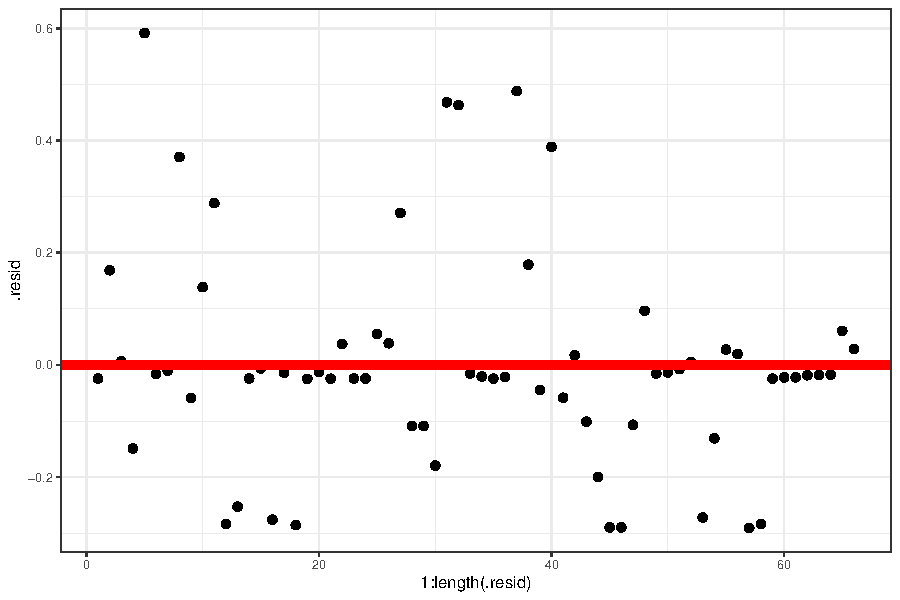
\includegraphics{index_files/figure-latex/unnamed-chunk-16-1.pdf}

Evaluación de los modelos: AIC, BIC y R2.

\begin{Shaded}
\begin{Highlighting}[]
\KeywordTok{glance}\NormalTok{(mod1)}
\end{Highlighting}
\end{Shaded}

\begin{verbatim}
## # A tibble: 1 x 12
##   r.squared adj.r.squared sigma statistic p.value    df logLik   AIC   BIC
##       <dbl>         <dbl> <dbl>     <dbl>   <dbl> <dbl>  <dbl> <dbl> <dbl>
## 1     0.325         0.315 0.196      30.9 5.74e-7     1   15.0 -24.0 -17.5
## # ... with 3 more variables: deviance <dbl>, df.residual <int>, nobs <int>
\end{verbatim}

\hypertarget{modelo-regresiuxf3n-lineal-sin-efectos-aleatorios}{%
\subsection{6.2. Modelo Regresión lineal sin efectos
aleatorios}\label{modelo-regresiuxf3n-lineal-sin-efectos-aleatorios}}

En este modelo utilizamos una fórmula sin el componente aleatorio. Un
modelo lineal simple

\begin{Shaded}
\begin{Highlighting}[]
\NormalTok{mod2 <-}\StringTok{ }\KeywordTok{lm}\NormalTok{(costos_gastos_totales }\OperatorTok{~}\StringTok{ }\NormalTok{estado }\OperatorTok{+}\StringTok{ }\NormalTok{ingresos_totales, }
           \DataTypeTok{data=}\NormalTok{ base_modelo_lineal) }
\KeywordTok{anova}\NormalTok{(mod2)}
\end{Highlighting}
\end{Shaded}

\begin{verbatim}
## Analysis of Variance Table
## 
## Response: costos_gastos_totales
##                  Df  Sum Sq Mean Sq F value    Pr(>F)    
## estado            1 1.18196 1.18196  51.004 1.131e-09 ***
## ingresos_totales  1 0.99111 0.99111  42.769 1.258e-08 ***
## Residuals        63 1.45995 0.02317                      
## ---
## Signif. codes:  0 '***' 0.001 '**' 0.01 '*' 0.05 '.' 0.1 ' ' 1
\end{verbatim}

\begin{Shaded}
\begin{Highlighting}[]
\KeywordTok{summary}\NormalTok{(mod2)}
\end{Highlighting}
\end{Shaded}

\begin{verbatim}
## 
## Call:
## lm(formula = costos_gastos_totales ~ estado + ingresos_totales, 
##     data = base_modelo_lineal)
## 
## Residuals:
##      Min       1Q   Median       3Q      Max 
## -0.25499 -0.04208 -0.01584  0.02511  0.47185 
## 
## Coefficients:
##                  Estimate Std. Error t value Pr(>|t|)    
## (Intercept)       -0.1120     0.0434  -2.580   0.0122 *  
## estadoVIGILANCIA   0.1881     0.0394   4.773 1.12e-05 ***
## ingresos_totales   0.9080     0.1389   6.540 1.26e-08 ***
## ---
## Signif. codes:  0 '***' 0.001 '**' 0.01 '*' 0.05 '.' 0.1 ' ' 1
## 
## Residual standard error: 0.1522 on 63 degrees of freedom
## Multiple R-squared:  0.5981, Adjusted R-squared:  0.5854 
## F-statistic: 46.89 on 2 and 63 DF,  p-value: 3.375e-13
\end{verbatim}

\begin{Shaded}
\begin{Highlighting}[]
\NormalTok{a <-}\StringTok{ }\KeywordTok{augment}\NormalTok{(mod2)}
\KeywordTok{ggplot}\NormalTok{(a, }\KeywordTok{aes}\NormalTok{(}\DataTypeTok{x=}\DecValTok{1}\OperatorTok{:}\KeywordTok{length}\NormalTok{(.resid), }\DataTypeTok{y=}\NormalTok{.resid))}\OperatorTok{+}
\StringTok{  }\KeywordTok{geom_point}\NormalTok{() }\OperatorTok{+}\StringTok{ }
\StringTok{  }\KeywordTok{geom_hline}\NormalTok{(}\DataTypeTok{yintercept =} \DecValTok{0}\NormalTok{, }\DataTypeTok{lwd=}\DecValTok{2}\NormalTok{, }\DataTypeTok{col=} \StringTok{"red"}\NormalTok{)}
\end{Highlighting}
\end{Shaded}

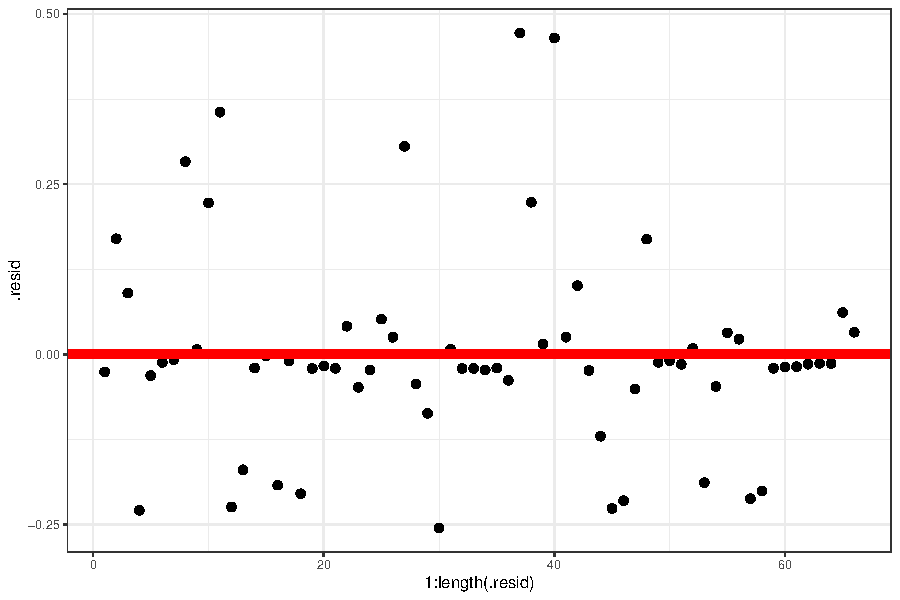
\includegraphics{index_files/figure-latex/unnamed-chunk-20-1.pdf}

Evaluación de los modelos: AIC, BIC y R2.

\begin{Shaded}
\begin{Highlighting}[]
\KeywordTok{glance}\NormalTok{(mod2)}
\end{Highlighting}
\end{Shaded}

\begin{verbatim}
## # A tibble: 1 x 12
##   r.squared adj.r.squared sigma statistic  p.value    df logLik   AIC   BIC
##       <dbl>         <dbl> <dbl>     <dbl>    <dbl> <dbl>  <dbl> <dbl> <dbl>
## 1     0.598         0.585 0.152      46.9 3.37e-13     2   32.1 -56.2 -47.5
## # ... with 3 more variables: deviance <dbl>, df.residual <int>, nobs <int>
\end{verbatim}

\hypertarget{modelo-lineal-con-intercepto-aleatorio}{%
\subsection{6.3. Modelo lineal con intercepto
aleatorio}\label{modelo-lineal-con-intercepto-aleatorio}}

En este modelo utilizamos una fórmula con el componente aleatorio por
departamento

\begin{Shaded}
\begin{Highlighting}[]
\KeywordTok{library}\NormalTok{(lme4)}
\NormalTok{mod4 <-}\StringTok{ }\KeywordTok{lmer}\NormalTok{(costos_gastos_totales }\OperatorTok{~}\StringTok{ }\NormalTok{ingresos_totales }\OperatorTok{+}\StringTok{ }\NormalTok{(}\DecValTok{1}\OperatorTok{|}\NormalTok{departamento), }
             \DataTypeTok{data=}\NormalTok{ base_modelo_lineal) }

\KeywordTok{anova}\NormalTok{(mod4)}
\end{Highlighting}
\end{Shaded}

\begin{verbatim}
## Analysis of Variance Table
##                  npar Sum Sq Mean Sq F value
## ingresos_totales    1 1.6452  1.6452  52.967
\end{verbatim}

\begin{Shaded}
\begin{Highlighting}[]
\KeywordTok{summary}\NormalTok{(mod4)}
\end{Highlighting}
\end{Shaded}

\begin{verbatim}
## Linear mixed model fit by REML ['lmerMod']
## Formula: costos_gastos_totales ~ ingresos_totales + (1 | departamento)
##    Data: base_modelo_lineal
## 
## REML criterion at convergence: -36.1
## 
## Scaled residuals: 
##     Min      1Q  Median      3Q     Max 
## -1.0611 -0.5900 -0.4911  0.3066  3.2155 
## 
## Random effects:
##  Groups       Name        Variance  Std.Dev. 
##  departamento (Intercept) 6.354e-23 7.971e-12
##  Residual                 3.106e-02 1.762e-01
## Number of obs: 66, groups:  departamento, 3
## 
## Fixed effects:
##                  Estimate Std. Error t value
## (Intercept)       0.02375    0.03796   0.626
## ingresos_totales  1.11269    0.15289   7.278
## 
## Correlation of Fixed Effects:
##             (Intr)
## ingrss_ttls 0.821 
## convergence code: 0
## boundary (singular) fit: see ?isSingular
\end{verbatim}

\begin{Shaded}
\begin{Highlighting}[]
\NormalTok{a <-}\StringTok{ }\NormalTok{broom.mixed}\OperatorTok{::}\KeywordTok{augment}\NormalTok{(mod4) }
\KeywordTok{ggplot}\NormalTok{(a, }\KeywordTok{aes}\NormalTok{(}\DataTypeTok{x=}\DecValTok{1}\OperatorTok{:}\KeywordTok{length}\NormalTok{(.resid), }\DataTypeTok{y=}\NormalTok{.resid))}\OperatorTok{+}
\StringTok{  }\KeywordTok{geom_point}\NormalTok{() }\OperatorTok{+}\StringTok{ }
\StringTok{  }\KeywordTok{geom_hline}\NormalTok{(}\DataTypeTok{yintercept =} \DecValTok{0}\NormalTok{, }\DataTypeTok{lwd=}\DecValTok{2}\NormalTok{, }\DataTypeTok{col=} \StringTok{"red"}\NormalTok{)}
\end{Highlighting}
\end{Shaded}

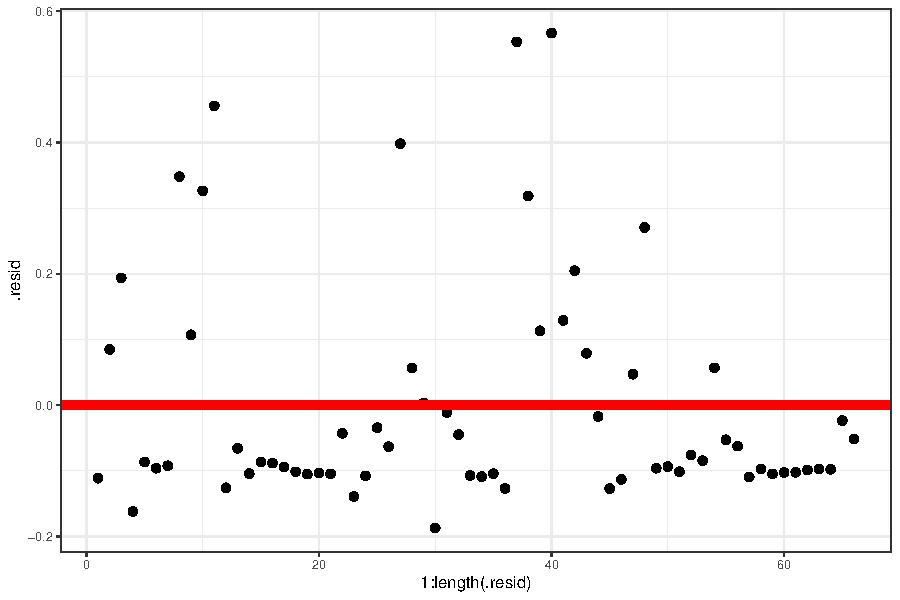
\includegraphics{index_files/figure-latex/unnamed-chunk-24-1.pdf}

Evaluación de los modelos: AIC, BIC y R2.

\begin{Shaded}
\begin{Highlighting}[]
\NormalTok{broom.mixed}\OperatorTok{::}\KeywordTok{glance}\NormalTok{(mod4)}
\end{Highlighting}
\end{Shaded}

\begin{verbatim}
## # A tibble: 1 x 6
##   sigma logLik   AIC   BIC REMLcrit df.residual
##   <dbl>  <dbl> <dbl> <dbl>    <dbl>       <int>
## 1 0.176   18.0 -28.1 -19.3    -36.1          62
\end{verbatim}

\hypertarget{modelo-lineal-con-intercepto-aleatorio-a-nivel-de-nit}{%
\subsection{6.4. Modelo Lineal con intercepto aleatorio a nivel de
NIT}\label{modelo-lineal-con-intercepto-aleatorio-a-nivel-de-nit}}

En este modelo utilizamos una fórmula con el componente aleatorio por
NIT, además contiene una interacción entre los ingresos totales y el
estado

\begin{Shaded}
\begin{Highlighting}[]
\KeywordTok{library}\NormalTok{(lme4)}
\NormalTok{mod5 <-}\StringTok{ }\KeywordTok{lmer}\NormalTok{(costos_gastos_totales }\OperatorTok{~}\StringTok{ }\KeywordTok{I}\NormalTok{(ingresos_totales)}\OperatorTok{:}\NormalTok{estado }\OperatorTok{+}\StringTok{  }\NormalTok{compra_Oro }
             \OperatorTok{+}\StringTok{ }\NormalTok{compra_Plata }\OperatorTok{+}\StringTok{ }\NormalTok{compra_Platino }\OperatorTok{+}\StringTok{ }\NormalTok{venta_Oro }\OperatorTok{+}\StringTok{ }\NormalTok{venta_Plata }\OperatorTok{+}\StringTok{ }
\StringTok{               }\NormalTok{venta_Platino }\OperatorTok{+}\StringTok{ }\NormalTok{ingresos_totales}\OperatorTok{+}\NormalTok{(}\DecValTok{1}\OperatorTok{|}\NormalTok{NIT), }
             \DataTypeTok{data=}\NormalTok{ base_modelo_lineal) }

\KeywordTok{anova}\NormalTok{(mod5)}
\end{Highlighting}
\end{Shaded}

\begin{verbatim}
## Analysis of Variance Table
##                            npar  Sum Sq Mean Sq F value
## compra_Oro                    1 0.00121 0.00121  0.1053
## compra_Plata                  1 0.00359 0.00359  0.3116
## ingresos_totales              1 0.38617 0.38617 33.5135
## I(ingresos_totales):estado    1 0.11916 0.11916 10.3416
\end{verbatim}

\begin{Shaded}
\begin{Highlighting}[]
\KeywordTok{summary}\NormalTok{(mod5)}
\end{Highlighting}
\end{Shaded}

\begin{verbatim}
## Linear mixed model fit by REML ['lmerMod']
## Formula: costos_gastos_totales ~ I(ingresos_totales):estado + compra_Oro +  
##     compra_Plata + compra_Platino + venta_Oro + venta_Plata +  
##     venta_Platino + ingresos_totales + (1 | NIT)
##    Data: base_modelo_lineal
## 
## REML criterion at convergence: -59.1
## 
## Scaled residuals: 
##      Min       1Q   Median       3Q      Max 
## -1.72445 -0.36330 -0.07757  0.08930  3.06148 
## 
## Random effects:
##  Groups   Name        Variance Std.Dev.
##  NIT      (Intercept) 0.01317  0.1148  
##  Residual             0.01152  0.1073  
## Number of obs: 66, groups:  NIT, 22
## 
## Fixed effects:
##                                      Estimate Std. Error t value
## (Intercept)                           0.07261    0.05017   1.447
## compra_Oro                           -0.01144    0.02220  -0.515
## compra_Plata                          0.01410    0.02218   0.636
## ingresos_totales                      0.89353    0.19598   4.559
## I(ingresos_totales):estadoINSPECCION  0.75545    0.23492   3.216
## 
## Correlation of Fixed Effects:
##             (Intr) cmpr_O cmpr_P ingrs_
## compra_Oro  -0.035                     
## compra_Plat  0.008 -0.799              
## ingrss_ttls  0.622 -0.048 -0.006       
## I(_):INSPEC  0.341  0.006  0.023 -0.300
## fit warnings:
## fixed-effect model matrix is rank deficient so dropping 5 columns / coefficients
\end{verbatim}

\begin{Shaded}
\begin{Highlighting}[]
\NormalTok{a <-}\StringTok{ }\NormalTok{broom.mixed}\OperatorTok{::}\KeywordTok{augment}\NormalTok{(mod5)}
\KeywordTok{ggplot}\NormalTok{(a, }\KeywordTok{aes}\NormalTok{(}\DataTypeTok{x=}\DecValTok{1}\OperatorTok{:}\KeywordTok{length}\NormalTok{(.resid), }\DataTypeTok{y=}\NormalTok{.resid))}\OperatorTok{+}
\StringTok{  }\KeywordTok{geom_point}\NormalTok{() }\OperatorTok{+}\StringTok{ }
\StringTok{  }\KeywordTok{geom_hline}\NormalTok{(}\DataTypeTok{yintercept =} \DecValTok{0}\NormalTok{, }\DataTypeTok{lwd=}\DecValTok{2}\NormalTok{, }\DataTypeTok{col=} \StringTok{"red"}\NormalTok{)}
\end{Highlighting}
\end{Shaded}

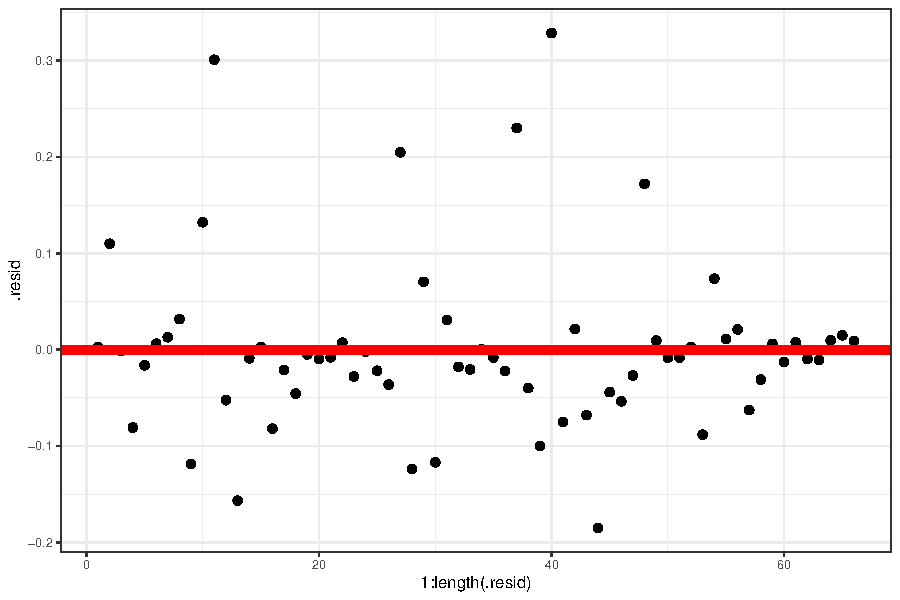
\includegraphics{index_files/figure-latex/unnamed-chunk-28-1.pdf}
Evaluación de los modelos: AIC, BIC y R2.

\begin{Shaded}
\begin{Highlighting}[]
\NormalTok{broom.mixed}\OperatorTok{::}\KeywordTok{glance}\NormalTok{(mod5)}
\end{Highlighting}
\end{Shaded}

\begin{verbatim}
## # A tibble: 1 x 6
##   sigma logLik   AIC   BIC REMLcrit df.residual
##   <dbl>  <dbl> <dbl> <dbl>    <dbl>       <int>
## 1 0.107   29.5 -45.1 -29.7    -59.1          59
\end{verbatim}

Se verificaron seis modelos. El primero, con una sola variable
explicativa llamada ``estado'' tiene un aporte al costo y al gasto de
forma positiva. Este modelo tiene un R2 de 19.85\% y un AIC de 74, lo
cual nos da el peor modelo. En el segundo modelo, se encuentra que,
agregando la variable de ingresos totales y el estado, el modelo
presenta un mejor ajuste para la explicación de los costos y gastos
(variable objetivo) para el sector minero. Este modelo tiene un R2 de
37.68\% y un AIC de 57, con lo cual obtenemos el mejor modelo. El
comportamiento de los residuales del modelo 2, también evidencian un
mejor comportamiento, al acercarse a cero. Para el tercer modelo, que es
el que tiene ``departamento'' evidenciamos que no es un modelo apropiado
para predecir los costos y gastos del sector minero, debido a que las
variables no son significativas. Los otros modelos evaluados, no
presentan mejoría al ingresarle las variables macroeconómicas
estandarizadas y ejecutar el modelo con efectos aleatorios en función de
cada compañía y/o el departamento. Por lo anterior, se selecciona como
un posible modelo el modelo número 2 \texttt{sin\ efecto\ aleatorio}, el
cual presenta el menor residual y mejor AIC.

\hypertarget{capuxedtulo-7.-estimaciuxf3n-de-esfuerzo}{%
\chapter{Capítulo 7. Estimación de
esfuerzo}\label{capuxedtulo-7.-estimaciuxf3n-de-esfuerzo}}

Para las actividades se realiza la siguiente estimación de esfuerzo:

\begin{enumerate}
\def\labelenumi{\arabic{enumi})}
\tightlist
\item
  Consolidación de información: 18h
\item
  Transformación de variables y análisis descriptivo: 10h
\item
  Ajuste y validación de modelos 15h
\item
  Redacción del reporte: 16h
\end{enumerate}

\hypertarget{capuxedtulo-8.-conclusiones}{%
\chapter{Capítulo 8. Conclusiones}\label{capuxedtulo-8.-conclusiones}}

\begin{itemize}
\tightlist
\item
  Para la variable objetivo propuesta ``costos\_gastos\_totales'', se
  evidencia que no es explicada por las variables macroeconómicas del
  país, dado que ésta no tiene un efecto volátil durante el año, sino
  que es constante. Este proceso se ve reflejado en el momento de
  evaluar las correlaciones con las variables sin transformar, así como
  con las variables estandarizadas.
\item
  Al adicionar variables económicas relacionadas al sector estudiado,
  como la compra y venta de materiales preciosos, no se evidencia que
  éstas expliquen, nuestra variable objetivo planteada.
\item
  El ejercicio de verificación con un modelo de regresión lineal simple,
  evidencia que ninguna variable, incluyendo las del sector son
  significativas, obteniendo modelos con R2 inferiores al 30\%,
  solamente quedando la variable ingresos totales como significativa.
\item
  Se recomieda para los datos trabajados, un acercamiento distinto.
\item
  Cuando los datos están concebidos y correlacionados históricamente,
  los modelos lineales mixtos son una herramienta muy robusta de
  análisis estadístico.
\end{itemize}

\hypertarget{referencias}{%
\chapter{REFERENCIAS}\label{referencias}}

\begin{itemize}
\item
  \url{https://www.dian.gov.co/ciiu/Documents/Resolucion_000139_21_Nov_2012.pdf}
\item
  \url{https://linea.ccb.org.co/descripcionciiu/}
\item
  \url{https://siis.ia.supersociedades.gov.co/}
\item
  \url{https://www.supersociedades.gov.co/delegatura_aec/Paginas/Base-completa-EF-2019.aspx}
\item
  \url{https://www.researchgate.net/publication/314536942_Introduccion_a_los_modelos_mixtos_Introduction_to_mixed_models}
\end{itemize}

\backmatter
\end{document}
